%%%%%%%%%%%%%%%%%%%%%%%%%%%%%%%%%%%%%%%%%%
% SECTION ENGLISH HANDWRITTEN CHARACTERS %
%%%%%%%%%%%%%%%%%%%%%%%%%%%%%%%%%%%%%%%%%%

\subsection{MNISTified Datasets}

To establish a baseline for the geometric properties of the in-distribution data, we first characterized the average padding and centring of each digit in the original MNIST dataset. This provides a basis for conforming the out-of-distribution handwritten characters to a similar format.

This section describes the processes used to conform the English Handwritten Character Dataset \cite{deCampos09} to the MNIST dataset, to provide the model trained on the MNIST dataset, data that may be visually similar (digits) but not always related (characters) to the original MNIST dataset (digits)
The English Handwritten Characters Dataset  contains 3,410 images of handwritten characters in English, 62 classes and 55 images of each class: 0-9, A-Z and a-z. There are 1430 uppercase characters, 1430 lowercase characters and 550 digits. Image are 1200 x 900 pixels in size, all RGB (3 channel) in PNG format. Figure \ref{fig:sample_handwritten_characters} shows a sample of 12 characters. 

% Repo git@github.com:dsikar/work-in-progress.git
% Script exploratory-handwritten-digits-sample-2.py
% commit 11f=0b9af
\begin{figure}[ht]
    \centering
    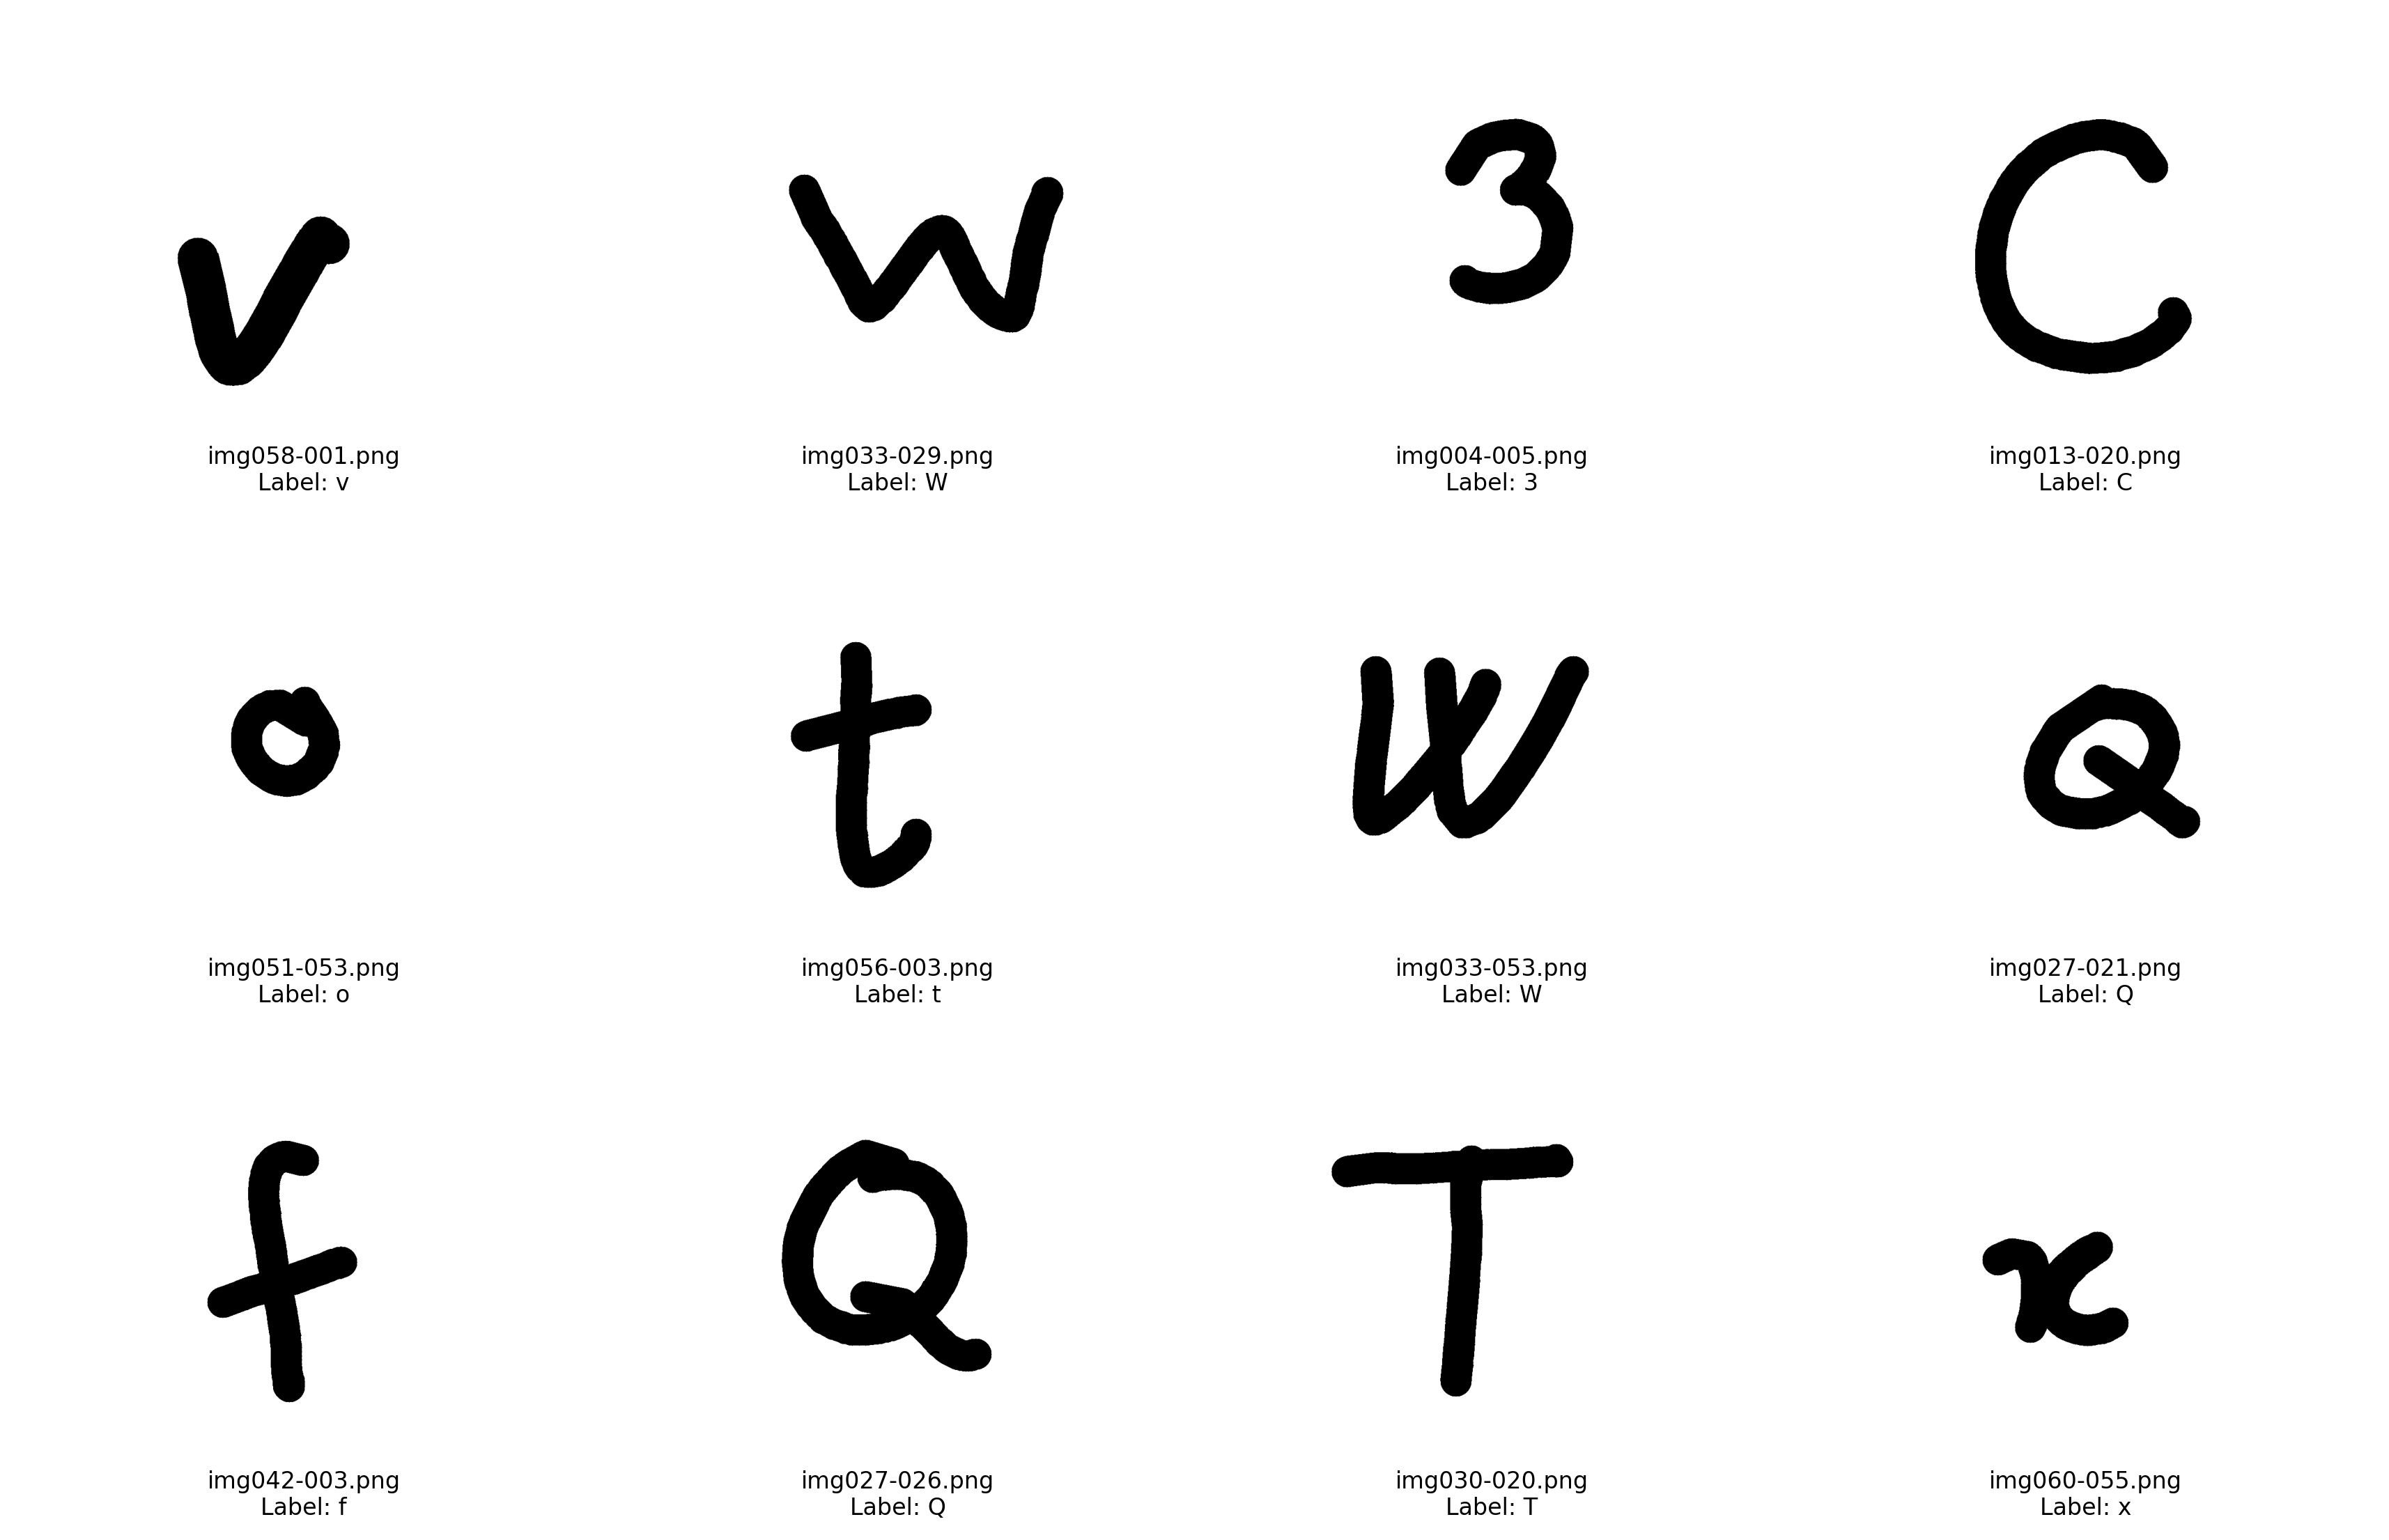
\includegraphics[width=0.99\columnwidth]{Figures/Results/HandwrittenCharacters/sample_handwritten_characters.png}
    \caption{Sample of handwritten digits from the Kaggle Handwritten Character Dataset}
\label{fig:sample_handwritten_characters}
\end{figure}

%%%%%%%%%%%%%%%%%%%%%%%%%%%%%
% PADDING STATISTICS TABLES %
%%%%%%%%%%%%%%%%%%%%%%%%%%%%%

\begin{table}[h]
\centering
\begin{tabular}{lcccccccccc}
Attribute & 0 & 1 & 2 & 3 & 4 & 5 & 6 & 7 & 8 & 9 \\
\hline
Left Padding (\%) & 19.88 & 35.18 & 19.57 & 18.88 & 22.26 & 21.97 & 26.65 & 20.19 & 25.12 & 24.80 \\
Right Padding (\%) & 15.81 & 31.44 & 15.17 & 22.27 & 19.23 & 13.83 & 18.96 & 22.54 & 18.29 & 24.12 \\
Top Padding (\%) & 15.97 & 15.46 & 14.09 & 16.49 & 17.85 & 18.65 & 8.97 & 24.35 & 17.32 & 22.29 \\
Bottom Padding (\%) & 14.16 & 13.14 & 17.04 & 12.54 & 11.17 & 13.44 & 19.81 & 4.70 & 11.62 & 6.36 \\
Left Padding (px) & 5.57 & 9.85 & 5.48 & 5.29 & 6.23 & 6.15 & 7.46 & 5.65 & 7.03 & 6.94 \\
Right Padding (px) & 4.43 & 8.80 & 4.25 & 6.24 & 5.38 & 3.87 & 5.31 & 6.31 & 5.12 & 6.75 \\
Top Padding (px) & 4.47 & 4.33 & 3.95 & 4.62 & 5.00 & 5.22 & 2.51 & 6.82 & 4.85 & 6.24 \\
Bottom Padding (px) & 3.97 & 3.68 & 4.77 & 3.51 & 3.13 & 3.76 & 5.55 & 1.32 & 3.25 & 1.78 \\
\end{tabular}
\caption{Training Set Padding Averages}
\label{app:MNIST_Training_Dataset_pixel_padding_stats}
\end{table}

\begin{table}[h]
\centering
\begin{tabular}{lcccccccccc}
Attribute & 0 & 1 & 2 & 3 & 4 & 5 & 6 & 7 & 8 & 9 \\
\hline
Left Padding (\%) & 20.25 & 35.91 & 19.78 & 19.48 & 22.23 & 21.95 & 26.00 & 20.49 & 25.53 & 24.78 \\
Right Padding (\%) & 15.91 & 31.92 & 15.52 & 22.69 & 19.69 & 13.87 & 17.97 & 23.06 & 18.80 & 24.10 \\
Top Padding (\%) & 15.94 & 15.49 & 13.93 & 16.42 & 17.96 & 18.61 & 8.92 & 24.00 & 17.27 & 22.21 \\
Bottom Padding (\%) & 14.39 & 13.09 & 16.72 & 12.63 & 11.00 & 13.21 & 19.86 & 4.90 & 11.62 & 6.40 \\
Left Padding (px) & 5.67 & 10.06 & 5.54 & 5.45 & 6.22 & 6.14 & 7.28 & 5.74 & 7.15 & 6.94 \\
Right Padding (px) & 4.46 & 8.94 & 4.34 & 6.35 & 5.51 & 3.88 & 5.03 & 6.46 & 5.26 & 6.75 \\
Top Padding (px) & 4.46 & 4.34 & 3.90 & 4.60 & 5.03 & 5.21 & 2.50 & 6.72 & 4.83 & 6.22 \\
Bottom Padding (px) & 4.03 & 3.66 & 4.68 & 3.54 & 3.08 & 3.70 & 5.56 & 1.37 & 3.25 & 1.79 \\
\end{tabular}
\caption{Testing Set Padding Averages}
\label{app:MNIST_Testing_Dataset_pixel_padding_stats}
\end{table}

We are interested in using our CNN trained on MNIST to predict the characters, then examine distances to predicted class centroids and compute statistics to establish if said distances help express uncertainty about characters that the network has not seen and does not know about e.g. letters of the alphabet.

Tables \ref{app:MNIST_Training_Dataset_pixel_padding_stats} and \ref{app:MNIST_Testing_Dataset_pixel_padding_stats} show padding as a percentage and average pixel value for training and testing datasets. It can be observed that in general digit 1 has larger left and right padding values compared to other digits. 
% discussion()
% MNIST_padding_stats.py
% commit 98f7eee
% repo git@github.com:dsikar/work-in-progress.git

Aggregate statistics for left, right, top, and bottom padding as percentages, including means and ranges, for the MNIST training and testing datasets:
\begin{itemize}
    \item \textbf{Training Set:}
    \begin{itemize}
        \item Left Padding: Mean = 23.45\%, Range = 18.88\% (digit 3) to 35.18\% (digit 1)
        \item Right Padding: Mean = 20.17\%, Range = 13.83\% (digit 5) to 31.44\% (digit 1)
        \item Top Padding: Mean = 17.14\%, Range = 8.97\% (digit 6) to 24.35\% (digit 7)
        \item Bottom Padding: Mean = 12.40\%, Range = 4.70\% (digit 7) to 19.81\% (digit 6)
    \end{itemize}
    \item \textbf{Testing Set:}
    \begin{itemize}
        \item Left Padding: Mean = 22.64\%, Range = 19.48\% (digit 3) to 35.91\% (digit 1)
        \item Right Padding: Mean = 20.35\%, Range = 13.87\% (digit 5) to 31.92\% (digit 1)
        \item Top Padding: Mean = 17.07\%, Range = 8.92\% (digit 6) to 24.00\% (digit 7)
        \item Bottom Padding: Mean = 12.38\%, Range = 4.90\% (digit 7) to 19.86\% (digit 6)
    \end{itemize}
\end{itemize}

% \begin{table}[h]
% \centering
% \begin{tabular}{lcccccccccc}
% Attribute & 0 & 1 & 2 & 3 & 4 & 5 & 6 & 7 & 8 & 9 \\
% \hline
% Left Padding (\%) & 20.25 & 35.91 & 19.78 & 19.48 & 22.23 & 21.95 & 26.00 & 20.49 & 25.53 & 24.78 \\
% Right Padding (\%) & 15.91 & 31.92 & 15.52 & 22.69 & 19.69 & 13.87 & 17.97 & 23.06 & 18.80 & 24.10 \\
% Top Padding (\%) & 15.94 & 15.49 & 13.93 & 16.42 & 17.96 & 18.61 & 8.92 & 24.00 & 17.27 & 22.21 \\
% Bottom Padding (\%) & 14.39 & 13.09 & 16.72 & 12.63 & 11.00 & 13.21 & 19.86 & 4.90 & 11.62 & 6.40 \\
% Left Padding (px) & 5.67 & 10.06 & 5.54 & 5.45 & 6.22 & 6.14 & 7.28 & 5.74 & 7.15 & 6.94 \\
% Right Padding (px) & 4.46 & 8.94 & 4.34 & 6.35 & 5.51 & 3.88 & 5.03 & 6.46 & 5.26 & 6.75 \\
% Top Padding (px) & 4.46 & 4.34 & 3.90 & 4.60 & 5.03 & 5.21 & 2.50 & 6.72 & 4.83 & 6.22 \\
% Bottom Padding (px) & 4.03 & 3.66 & 4.68 & 3.54 & 3.08 & 3.70 & 5.56 & 1.37 & 3.25 & 1.79 \\
% \end{tabular}
% \caption{Testing Set Padding Averages}
% \label{app:MNIST_Testing_Dataset_pixel_padding_stats}
% \end{table}

% MNIST_padding_stats
% git@github.com:dsikar/work-in-progress.git

% Should be the same as previous tables
% \begin{table}[h]
% \centering
% \begin{tabular}{lcccccccccc}
% Attribute & 0 & 1 & 2 & 3 & 4 & 5 & 6 & 7 & 8 & 9 \\
% \hline
% Left Padding (\%) & 19.88 & 35.18 & 19.57 & 18.88 & 22.26 & 21.97 & 26.65 & 20.19 & 25.12 & 24.80 \\
% Right Padding (\%) & 15.81 & 31.44 & 15.17 & 22.27 & 19.23 & 13.83 & 18.96 & 22.54 & 18.29 & 24.12 \\
% Top Padding (\%) & 15.97 & 15.46 & 14.09 & 16.49 & 17.85 & 18.65 & 8.97 & 24.35 & 17.32 & 22.29 \\
% Bottom Padding (\%) & 14.16 & 13.14 & 17.04 & 12.54 & 11.17 & 13.44 & 19.81 & 4.70 & 11.62 & 6.36 \\
% Left Padding (px) & 5.57 & 9.85 & 5.48 & 5.29 & 6.23 & 6.15 & 7.46 & 5.65 & 7.03 & 6.94 \\
% Right Padding (px) & 4.43 & 8.80 & 4.25 & 6.24 & 5.38 & 3.87 & 5.31 & 6.31 & 5.12 & 6.75 \\
% Top Padding (px) & 4.47 & 4.33 & 3.95 & 4.62 & 5.00 & 5.22 & 2.51 & 6.82 & 4.85 & 6.24 \\
% Bottom Padding (px) & 3.97 & 3.68 & 4.77 & 3.51 & 3.13 & 3.76 & 5.55 & 1.32 & 3.25 & 1.78 \\
% \end{tabular}
% \caption{Training Set Padding Averages}
% \end{table}




% Perturbed testing dataset
% \begin{table}[h]
% \centering
% \begin{tabular}{lcccccccccc}
% Attribute & 0 & 1 & 2 & 3 & 4 & 5 & 6 & 7 & 8 & 9 \\
% \hline
% Left Padding (\%) & 5.82 & 10.89 & 5.55 & 5.41 & 6.33 & 6.27 & 7.77 & 5.71 & 7.67 & 7.25 \\
% Right Padding (\%) & 3.54 & 8.76 & 3.43 & 5.86 & 4.75 & 2.89 & 4.20 & 5.88 & 4.60 & 6.30 \\
% Top Padding (\%) & 3.47 & 3.05 & 2.62 & 3.51 & 3.97 & 4.27 & 0.99 & 6.18 & 3.85 & 5.54 \\
% Bottom Padding (\%) & 2.46 & 1.78 & 3.17 & 1.79 & 1.25 & 1.99 & 4.17 & 0.30 & 1.47 & 0.44 \\
% Left Padding (px) & 1.63 & 3.05 & 1.55 & 1.52 & 1.77 & 1.76 & 2.18 & 1.60 & 2.15 & 2.03 \\
% Right Padding (px) & 0.99 & 2.45 & 0.96 & 1.64 & 1.33 & 0.81 & 1.18 & 1.65 & 1.29 & 1.76 \\
% Top Padding (px) & 0.97 & 0.85 & 0.73 & 0.98 & 1.11 & 1.20 & 0.28 & 1.73 & 1.08 & 1.55 \\
% Bottom Padding (px) & 0.69 & 0.50 & 0.89 & 0.50 & 0.35 & 0.56 & 1.17 & 0.08 & 0.41 & 0.12 \\
% \end{tabular}
% \caption{Testing Set Padding Averages}
% \label{app:MNIST_Testing_Dataset_pixel_padding_stats}
% \end{table}


%\subsection{Single digit stats}

% single_image_stats(img_np)
% Repo git@github.com:dsikar/work-in-progress.git
% Script MNIST_padding_stats.py

%%%%%%%%%%%%%%%%%%%%%%
% SINGLE DIGIT STATS %
%%%%%%%%%%%%%%%%%%%%%%

Figure \ref{fig:MNIST_training_index_0_label_5} shows the first digit in the MNIST training dataset. The padding statistics for left, right, top and bottom are 4, 4, 5, 3 pixels respectively, and 14.29\%, 14.29\%, 17.86\%, 10.71\% as proportions of the 28x28 size.

% [(14.285714285714285, 14.285714285714285, 17.857142857142858, 10.714285714285714, 4, 4, 5, 3)]})

%%%%%%%%%%%
% DIGIT 5 %
%%%%%%%%%%%
\begin{figure}[ht]
    \centering
    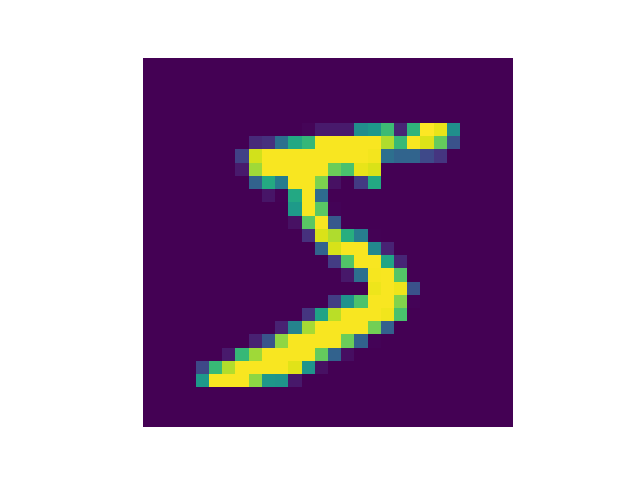
\includegraphics[width=0.50\columnwidth]{Figures/Results/HandwrittenCharacters/MNIST_training_index_0_label_5.png}
    \caption{MNIST Training example index 0 (first example), label 5}
\label{fig:MNIST_training_index_0_label_5}
\end{figure}

Figure \ref{fig:Training_Digits_1_5} shows a random selection of training data that reflects the general trends shows in tables \ref{app:MNIST_Training_Dataset_pixel_padding_stats} and \ref{app:MNIST_Testing_Dataset_pixel_padding_stats}, e.g. digit 1 typically has wider left and right paddings compared to digit 5.

%%%%%%%%%%%%%%%%%%%%%%
% DIGIT 1 AND 5 ROWS %
%%%%%%%%%%%%%%%%%%%%%%

% MNIST_training_testing_ones.py

\begin{figure}[ht]
    \centering
    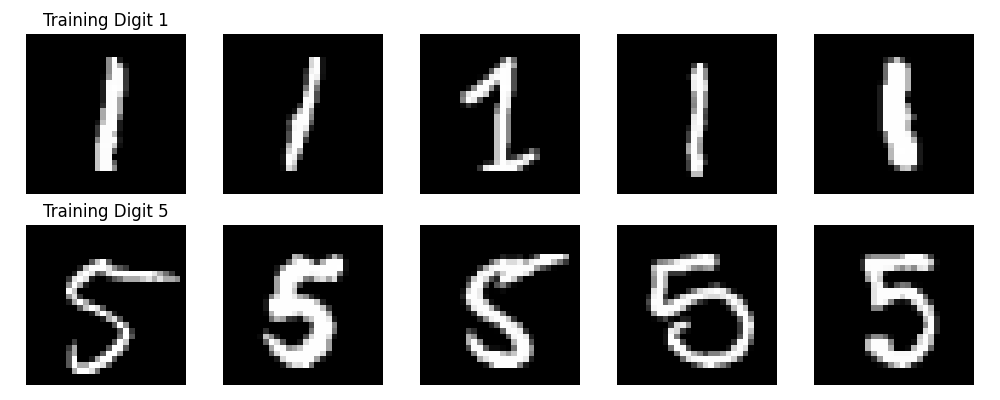
\includegraphics[width=0.99\columnwidth]{Figures/Results/HandwrittenCharacters/Training_Digits_1_5.png}
    \caption{Random selection of MNIST training data digits 1 on top row and 5 on bottom row}
\label{fig:Training_Digits_1_5}
\end{figure}

The left and top padding percentages in the MNIST training and testing datasets, as depicted in Figure \ref{fig:MNIST_training_testing_padding_plots}, reveal distinct trends across digits 0–9 that reflect the structural characteristics of handwritten digits. For left padding, both sets show a pronounced peak for digit 1 (training: 35.18\%, testing: 35.91\%), driven by its narrow, vertical shape, which leaves substantial horizontal space. This trend is consistent across sets, though testing values are slightly higher (e.g., 35.91\% vs. 35.18\%), suggesting minor positional variations. Other digits, such as 3 and 5, exhibit lower left padding (around 18–22\%), indicating wider or more centered shapes. Top padding, in contrast, shows greater variability, with digit 7 displaying the highest values (training: 24.35\%, testing: 24.00\%), reflecting its top-heavy strokes, while digit 6 has the lowest (training: 8.97\%, testing: 8.92\%), aligning with its bottom-heavy features. Across both padding types, training and testing sets are closely aligned, with mean differences under 1\% (left: 23.45\% vs. 22.64\%; top: 17.14\% vs. 17.07\%). 

%%%%%%%%%%%%%%%%%%%%%%%%%%%%%%%%%%%%
% MNIST LEFT AND TOP PADDING PLOTS %
%%%%%%%%%%%%%%%%%%%%%%%%%%%%%%%%%%%%

\begin{figure}[ht]
    \centering
    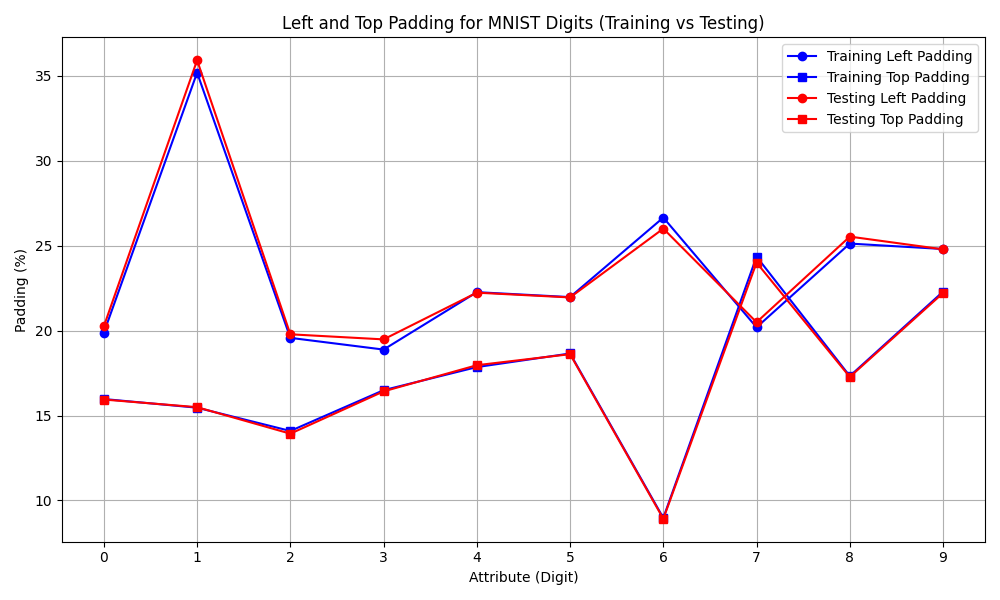
\includegraphics[width=0.99\columnwidth]{Figures/Results/HandwrittenCharacters/MNIST_training_testing_padding_plots.png}
    \caption{MNIST training and testing data left and top padding percentages i.e. padding in pixels / width|height (28 pixels)}
\label{fig:MNIST_training_testing_padding_plots}
\end{figure}

%\subsection{Converting the English Handwritten Characters to MNIST-like format}

%%%%%%%%%%%%%%%%%%%%%%%%%%%%%%%%%%%%%%%%%%%%%%%%%%%%%%%%%%%%%%%%%%%%%%
% CONVERTING the ENGLISH HANDWRITTEN CHARACTERS TO MNIST-LIKE FORMAT %
%%%%%%%%%%%%%%%%%%%%%%%%%%%%%%%%%%%%%%%%%%%%%%%%%%%%%%%%%%%%%%%%%%%%%%

The English Handwritten Characters dataset as previously mentioned are 1200 x 900 pixels in size, all RGB (3 channel) in PNG format, and need to be converted to 28x28 single channel grayscale images.

% Image Img/img004-005.png - Label: 3, Size: (1200, 900), Min/Max Pixel (grayscale): 0/255
% Image Img/img013-020.png - Label: C, Size: (1200, 900), Min/Max Pixel (grayscale): 0/255
% Image Img/img051-053.png - Label: o, Size: (1200, 900), Min/Max Pixel (grayscale): 0/255
% Image Img/img056-003.png - Label: t, Size: (1200, 900), Min/Max Pixel (grayscale): 0/255
% Image Img/img033-053.png - Label: W, Size: (1200, 900), Min/Max Pixel (grayscale): 0/255
% Image Img/img027-021.png - Label: Q, Size: (1200, 900), Min/Max Pixel (grayscale): 0/255
% Image Img/img042-003.png - Label: f, Size: (1200, 900), Min/Max Pixel (grayscale): 0/255
% Image Img/img027-026.png - Label: Q, Size: (1200, 900), Min/Max Pixel (grayscale): 0/255
% Image Img/img030-020.png - Label: T, Size: (1200, 900), Min/Max Pixel (grayscale): 0/255
% Image Img/img060-055.png - Label: x, Size: (1200, 900), Min/Max Pixel (grayscale): 0/255

% Padding for image (left%, right%, top%, bottom%, leftpx, rightpx, toppx, bottompx): (27.666666666666668, 41.833333333333336, 46.22222222222222, 13.777777777777779, 332, 502, 416, 124)
% Padding for image (left%, right%, top%, bottom%, leftpx, rightpx, toppx, bottompx): (30.666666666666664, 20.75, 36.333333333333336, 26.333333333333332, 368, 249, 327, 237)
% Padding for image (left%, right%, top%, bottom%, leftpx, rightpx, toppx, bottompx): (41.75, 35.5, 23.22222222222222, 33.0, 501, 426, 209, 297)
% Padding for image (left%, right%, top%, bottom%, leftpx, rightpx, toppx, bottompx): (30.416666666666664, 31.25, 23.333333333333332, 16.555555555555557, 365, 375, 210, 149)
% Padding for image (left%, right%, top%, bottom%, leftpx, rightpx, toppx, bottompx): (37.166666666666664, 43.5, 36.22222222222222, 37.666666666666664, 446, 522, 326, 339)
% Padding for image (left%, right%, top%, bottom%, leftpx, rightpx, toppx, bottompx): (31.0, 44.0, 25.666666666666664, 16.22222222222222, 372, 528, 231, 146)
% Padding for image (left%, right%, top%, bottom%, leftpx, rightpx, toppx, bottompx): (25.416666666666664, 32.75, 28.999999999999996, 27.88888888888889, 305, 393, 261, 251)
% Padding for image (left%, right%, top%, bottom%, leftpx, rightpx, toppx, bottompx): (38.916666666666664, 29.75, 35.66666666666667, 27.88888888888889, 467, 357, 321, 251)
% Padding for image (left%, right%, top%, bottom%, leftpx, rightpx, toppx, bottompx): (32.916666666666664, 40.5, 22.555555555555557, 15.666666666666668, 395, 486, 203, 141)
% Padding for image (left%, right%, top%, bottom%, leftpx, rightpx, toppx, bottompx): (29.416666666666668, 33.416666666666664, 22.333333333333332, 22.88888888888889, 353, 401, 201, 206)
% Padding for image (left%, right%, top%, bottom%, leftpx, rightpx, toppx, bottompx): (21.666666666666668, 35.5, 23.333333333333332, 17.0, 260, 426, 210, 153)
% Padding for image (left%, right%, top%, bottom%, leftpx, rightpx, toppx, bottompx): (31.666666666666664, 42.41666666666667, 44.0, 28.888888888888886, 380, 509, 396, 260)
% Average Left Padding %: 31.56, Range: 21.67–41.75

%%%%%%%%%%%%%%%%%
% PREPROCESSING %
%%%%%%%%%%%%%%%%%

Figure \ref{fig:english-handwritten-chracters-dataset-preprocessing} shows the preprocessing pipeline applied to the English handwritten characters dataset before neural network inference. The raw input character is 900×1200 pixels.

The pipeline standardizes an image for MNIST compatibility (28x28 pixels). It first verifies the input is a two-dimensional grayscale array. A threshold identifies foreground pixels, and the minimal bounding box is computed. The image is cropped to isolate the character. A scale factor is then calculated so that the longer side of the cropped region measures 22 pixels, preserving the original aspect ratio. The cropped image is resized using Lanczos resampling with this scale factor. Next, the pixel intensities are inverted, yielding a white character on a black background. Finally, the resized image is centered on a 28×28 canvas, producing the final MNIST-formatted image that aligns with the MNIST format used during the network's training phase


% he image is then cropped to remove excess whitespace, focusing only on the character itself. This cropped image varies in size depending on the character's shape and writing style. Next, the image is resized to 22×22 pixels using Lanczos resampling to preserve visual features while reducing dimensionality. In the final step, the image is inverted (changing black to white and vice versa) and padded with a 3-pixel border on all sides to create a standardized 28×28 pixel image. This standardization ensures the images match the input dimensions expected by the CNN, which has been trained on the MNIST dataset. The final inverted format, with the character appearing as white on a black background, aligns with the MNIST format used during the network's training phase.

% convert2MNISTFormat.ipynb
% Sample MNISTified images
% commit 03351e7

% import matplotlib.pyplot as plt
% import numpy as np

% # Data from the tables for Left Padding (%) for digits 0–9
% attributes = range(10)  # Digits 0 to 9
% training_left_padding = [19.88, 35.18, 19.57, 18.88, 22.26, 21.97, 26.65, 20.19, 25.12, 24.80]
% testing_left_padding = [20.25, 35.91, 19.78, 19.48, 22.23, 21.95, 26.00, 20.49, 25.53, 24.78]

% # Create the plot
% plt.figure(figsize=(10, 6))
% plt.plot(attributes, training_left_padding, 'b-o', label='Training Left Padding')
% plt.plot(attributes, testing_left_padding, 'r-o', label='Testing Left Padding')

% # Set labels and title
% plt.xlabel('Attribute (Digit)')
% plt.ylabel('Padding (%)')
% plt.title('Left Padding for MNIST Digits (Training vs Testing)')

% # Add legend
% plt.legend()

% # Add grid
% plt.grid(True)

% # Set x-ticks to show all integers 0–9
% plt.xticks(range(10))

% # Adjust layout and display
% plt.tight_layout()
% plt.show()

\begin{figure}[ht]
    \centering
    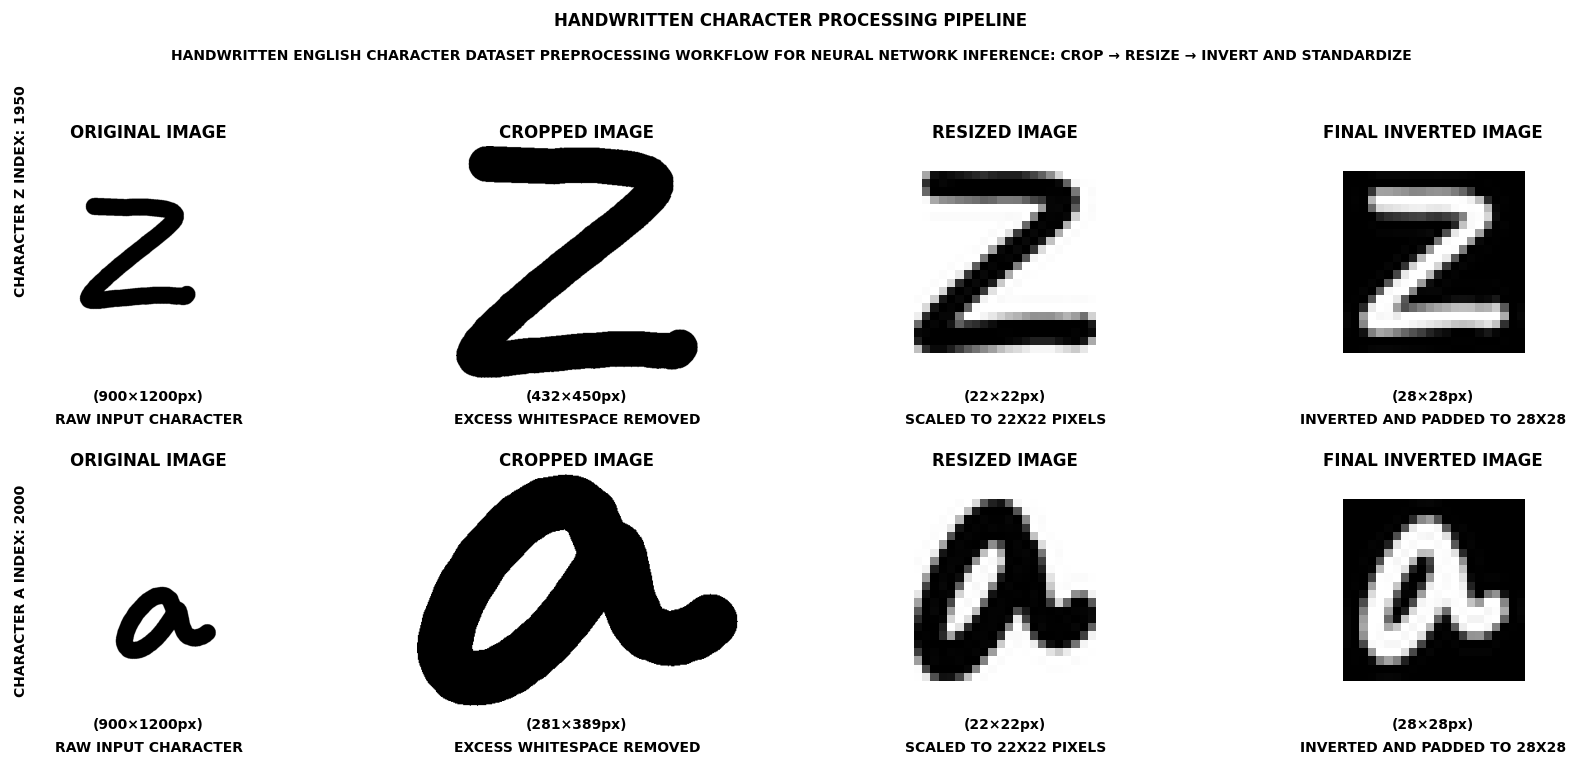
\includegraphics[width=0.99\columnwidth]{Figures/Results/HandwrittenCharacters/english-handwritten-chracters-dataset-preprocessing.png}
    \caption{Handwritten English Character Dataset "MNISTification" process, left to right, raw input character, character with excess white space removed, scaled (custom, based on character), and inverted (white font on black background), conforming to MNIST 28x28 pixel grayscale images.}
\label{fig:english-handwritten-chracters-dataset-preprocessing}
\end{figure}

Figures \ref{fig:mnistified-0-9}, \ref{fig:mnistified-A-Z} and \ref{fig:mnistified-a-z} shows samples of digits and upper and lower characters, processed to resemble the MNIST dataset.

% stopped here
% todos
% 1. processed digits 0 to 9, plot row OK
% 2. full alphabet lowercase, plot OK
% 3. full alphabe lowercase, plot OK
% 4. publish dataset
% 5. predict OK Accuracy 0.8727272727272727 (digits only)
% 6. softmax distances for digits correct / incorrect predictions
% 7. softmax distances for characters incorrect predictions nb correct N/A

%%%%%%%%%%%%%%%%%%%%%%%%%%%%%%%%%%%%%%%%%%%%%%%%%
% MNISTified English Handwritten Characters 0-9 %
%%%%%%%%%%%%%%%%%%%%%%%%%%%%%%%%%%%%%%%%%%%%%%%%%

% convert2MNISTFormat.ipynb - 0-9
% Sample MNISTified images
% commit 03351e7
\begin{figure}[ht]
    \centering
    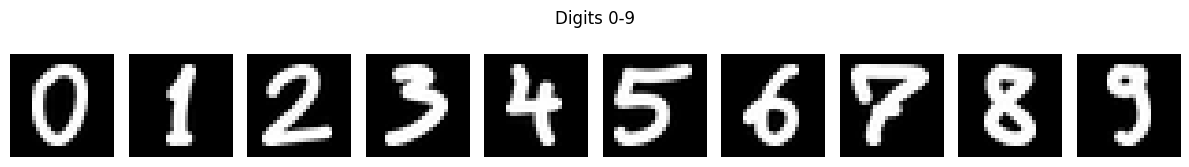
\includegraphics[width=0.99\columnwidth]{Figures/Results/HandwrittenCharacters/mnistified-0-9.png}
    \caption{MNISTified English Handwritten Characters 0-9}
\label{fig:mnistified-0-9}
\end{figure}


%%%%%%%%%%%%%%%%%%%%%%%%%%%%%%%%%%%%%%%%%%%%%%%%%
% MNISTified English Handwritten Characters A-Z %
%%%%%%%%%%%%%%%%%%%%%%%%%%%%%%%%%%%%%%%%%%%%%%%%%

% convert2MNISTFormat.ipynb - A-Z
% Sample MNISTified images
% commit 03351e7
\begin{figure}[ht]
    \centering
    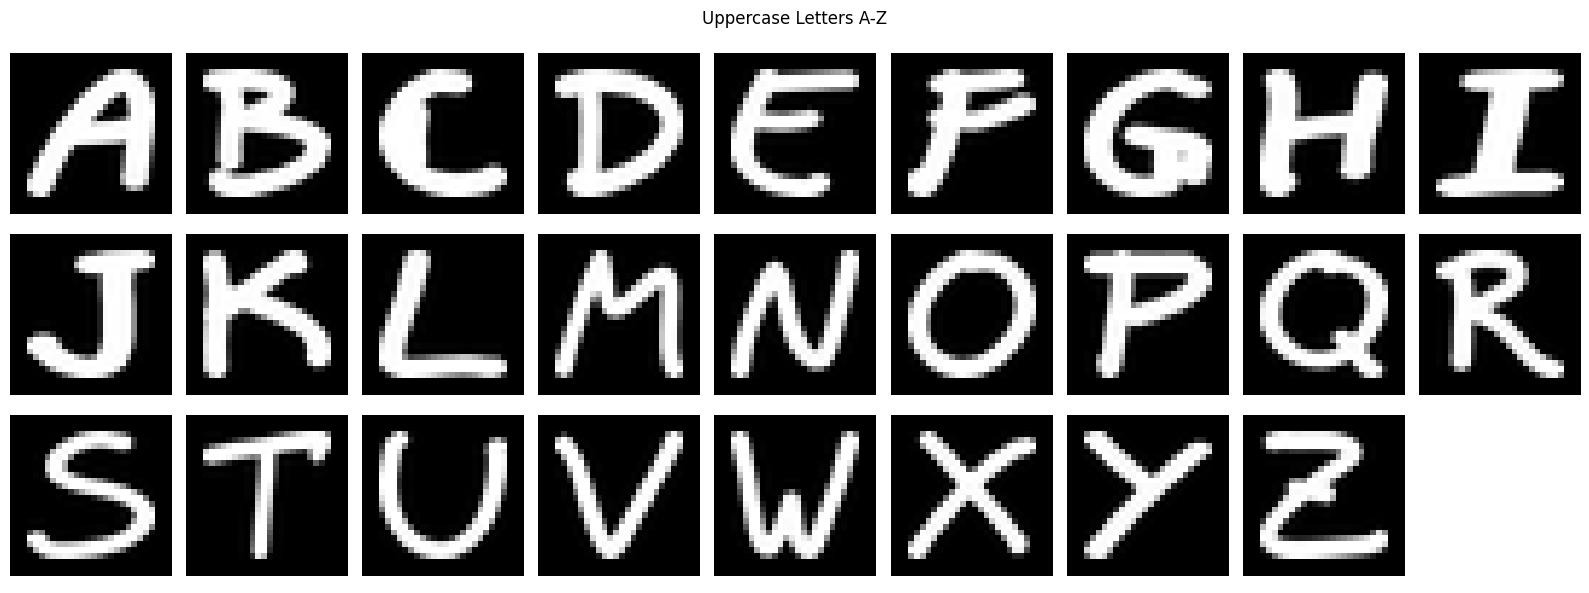
\includegraphics[width=0.99\columnwidth]{Figures/Results/HandwrittenCharacters/mnistified-A-Z.png}
    \caption{MNISTified English Handwritten Characters A-Z}
\label{fig:mnistified-A-Z}
\end{figure}


%%%%%%%%%%%%%%%%%%%%%%%%%%%%%%%%%%%%%%%%%%%%%%%%%
% MNISTified English Handwritten Characters a-z %
%%%%%%%%%%%%%%%%%%%%%%%%%%%%%%%%%%%%%%%%%%%%%%%%%

% convert2MNISTFormat.ipynb - a-z
% Sample MNISTified images
% commit 03351e7
\begin{figure}[ht]
    \centering
    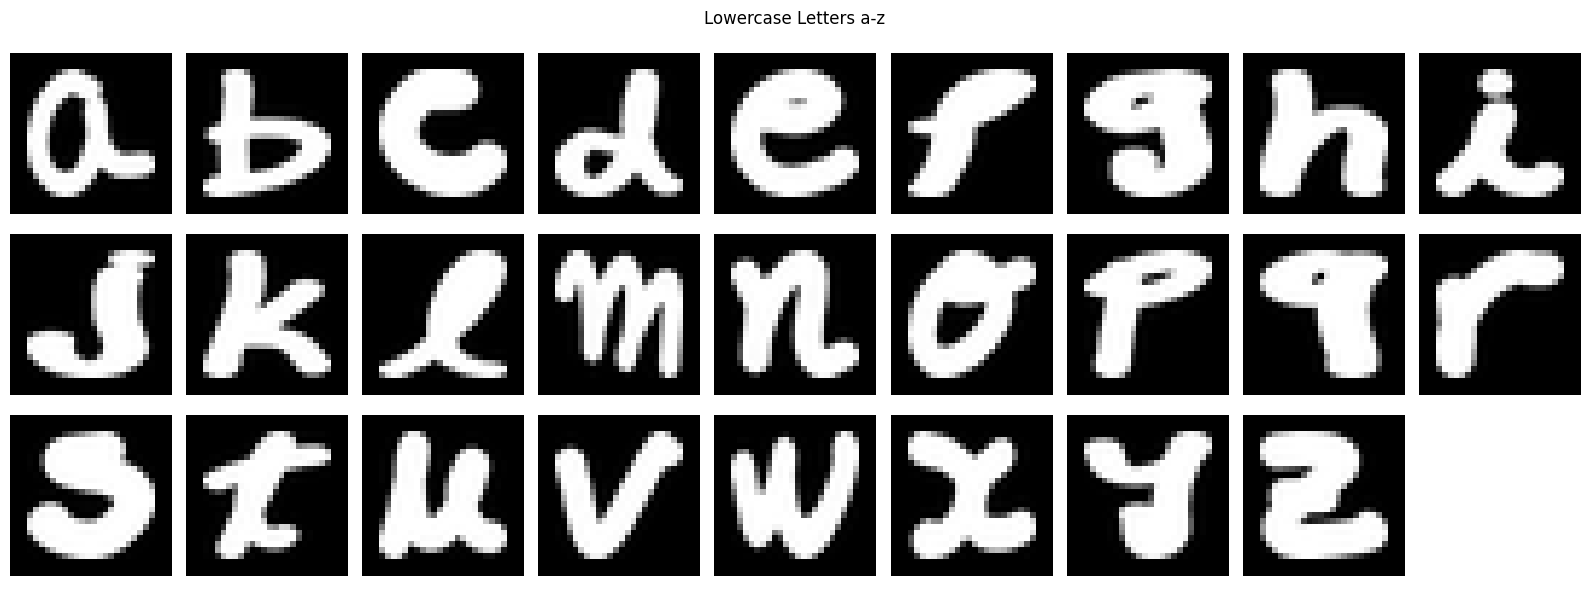
\includegraphics[width=0.99\columnwidth]{Figures/Results/HandwrittenCharacters/mnistified-a-z.png}
    \caption{MNISTified English Handwritten Characters a-z}
\label{fig:mnistified-a-z}
\end{figure}


%%%%%%%%%%%%%%%%%%%%%%%%%%%%%%%%%%%%%%%%%%
% HWC x MNIST LEFT AND TOP PADDING PLOTS %
%%%%%%%%%%%%%%%%%%%%%%%%%%%%%%%%%%%%%%%%%%

Figure \ref{fig:EHC_x_MNIST_training_testing_padding_plots} that digits 1, 9, and 8, in that order, exhibit the highest left-padding percentages, indicating they are narrower and thus need more horizontal space on the left to be centred. By contrast, 2, 1, and 5 are among the widest digits and therefore require less left padding. The top-padding values are relatively consistent across all digits, showing minimal variation in how they are positioned vertically. The MNISTified dataset is somewhat conformed to the MNIST dataset with respect to left padding, and also to right padding as can be observed in Figure \ref{fig:mnistified-0-9}.

% English_Handwritten_Charater_Digits_Padding_Stats.py
% plot_combined_padding(averages)
% commit 9906d82

\begin{figure}[ht]
    \centering
    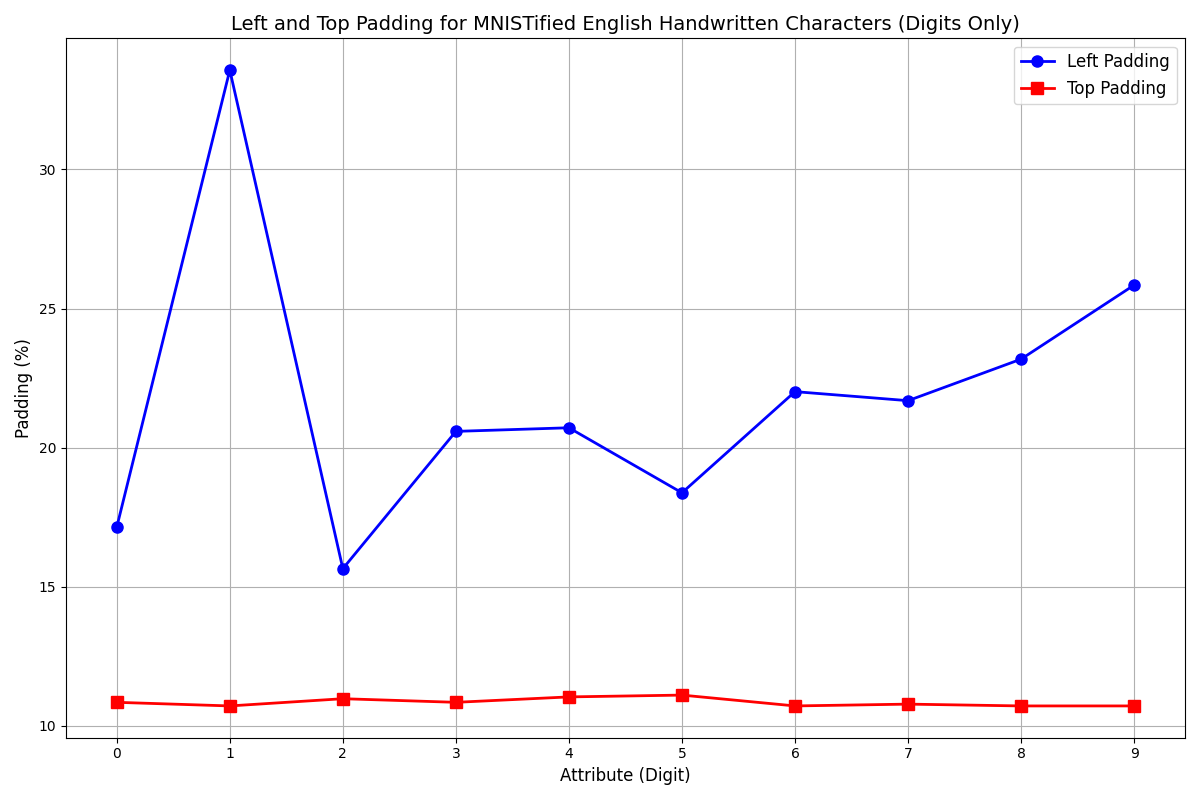
\includegraphics[width=0.99\columnwidth]{Figures/Results/HandwrittenCharacters/EHC_x_MNIST_training_testing_padding_plots.png}
    \caption{English Handwritten Characters (digits only) dataset conformed to MNIST layout}
\label{fig:EHC_x_MNIST_training_testing_padding_plots}
\end{figure}

%\subsection{MNISTified English Handwritten Character Results}

%%%%%%%%%%%%%%%%%%%%%%%%%%%%%%%%%%%%%%%%%%%%%%%%%%%%
% MNISTIFIED ENGLISH HANDWRITTEN CHARACTER RESULTS %
%%%%%%%%%%%%%%%%%%%%%%%%%%%%%%%%%%%%%%%%%%%%%%%%%%%%

Once conformed to the MNIST dataset, such that a trained CNN can be used for inference, the obtained accuracy on the English Handwritten Character digits is 87\%, compared to 98\% on the MNIST training dataset. 

Figure \ref{fig:english_handwritten_characters_digits_only_thresholds} shows the nearest distances (thresholds) for a class being misclassified e.g. the nearest misclassified digit 3 to digit 3 class centroid is 1.114 units away, and the nearest digit misclassified as a 6 is 0.251 units away from the 6 digit class centroid. Note there are no bars (blue or red) for digit 0 as no digit 0 was misclassified as another digit, and no other digits were misclassified as digit 0. Other similar cases are digits 2 and 5 (all digits correctly classified) and digit 4 (no digits misclassified as four), as can be seen in Figure \ref{fig:english_handwritten_characters_digits_only_confusion_matrix}, the confusion matrix for the MNISTified English Handwritten Character Dataset (Digits Only - 550 examples). 



The confusion matrix (Image 1) indicates high diagonal values, showing the model's accuracy for digit classification. Digits 0, 1, 2, 5, and 8 exhibit classification accuracy exceeding 95\%. The digit 7 displays significant misclassification patterns, with 10 instances classified as digit 3, 7 as digit 2, and 4 as digit 8. Digit 6 shows 14 cases misclassified as digit 5.
The threshold comparison (Image 2) presents distances of misclassified points on a logarithmic scale. The "Same Class" thresholds (blue) represent distances for points belonging to a class but misclassified elsewhere, while "Different Class" thresholds (red) show distances for points incorrectly assigned to a class. The largest disparity occurs for digits 4 and 5, where Different Class thresholds are minimal (0.007). Digits 6 and 9 demonstrate the highest Different Class thresholds (0.251 and 0.270), indicating more complex decision boundaries for these classes.

% ggit@github.com:dsikar/IJCNN-2025.git  mnist_alphabetic_character_analysis.py
% commit 91c8cc0
% Function call
% plot_thresholds_comparison(thresholds_same, thresholds_different, prefix="English Handwritten Characters Digits Only ", filename="english_handwritten_characters_digits_only_thresholds.png", save=True)
% # Saved as english_handwritten_characters_digits_only_thresholds.png
\begin{figure}[ht]
    \centering
    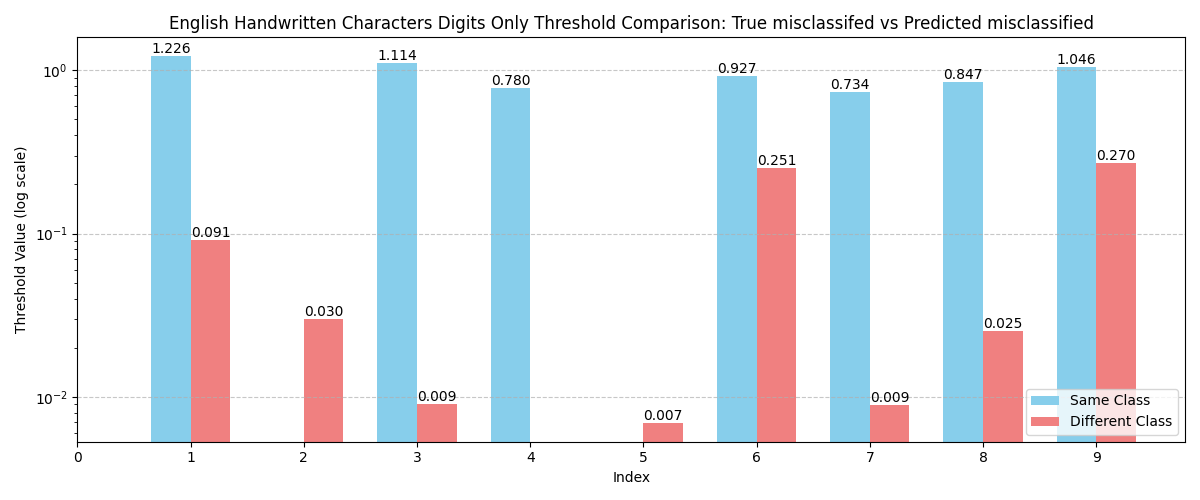
\includegraphics[width=0.99\columnwidth]{Figures/Results/HandwrittenCharacters/english_handwritten_characters_digits_only_thresholds.png}
    \caption{English Handwritten Characters (digits only) distances to class centroids, nearest "misprediction" of the true class (blue bars) and nearest misprediction of a predicted class}
\label{fig:english_handwritten_characters_digits_only_thresholds}
\end{figure}

% Function call
% # Confusion matrix for digits only
% confusion_matrix_digits = confusion_matrix(data_np, digits_only=True)
% plot_confusion_matrix(confusion_matrix_digits, prefix="English Handwritten Characters Digits Only ", filename="english_handwritten_characters_digits_only_confusion_matrix.png", save=True)
% # Saved as english_handwritten_characters_digits_only_confusion_matrix.png
\begin{figure}[ht]
    \centering
    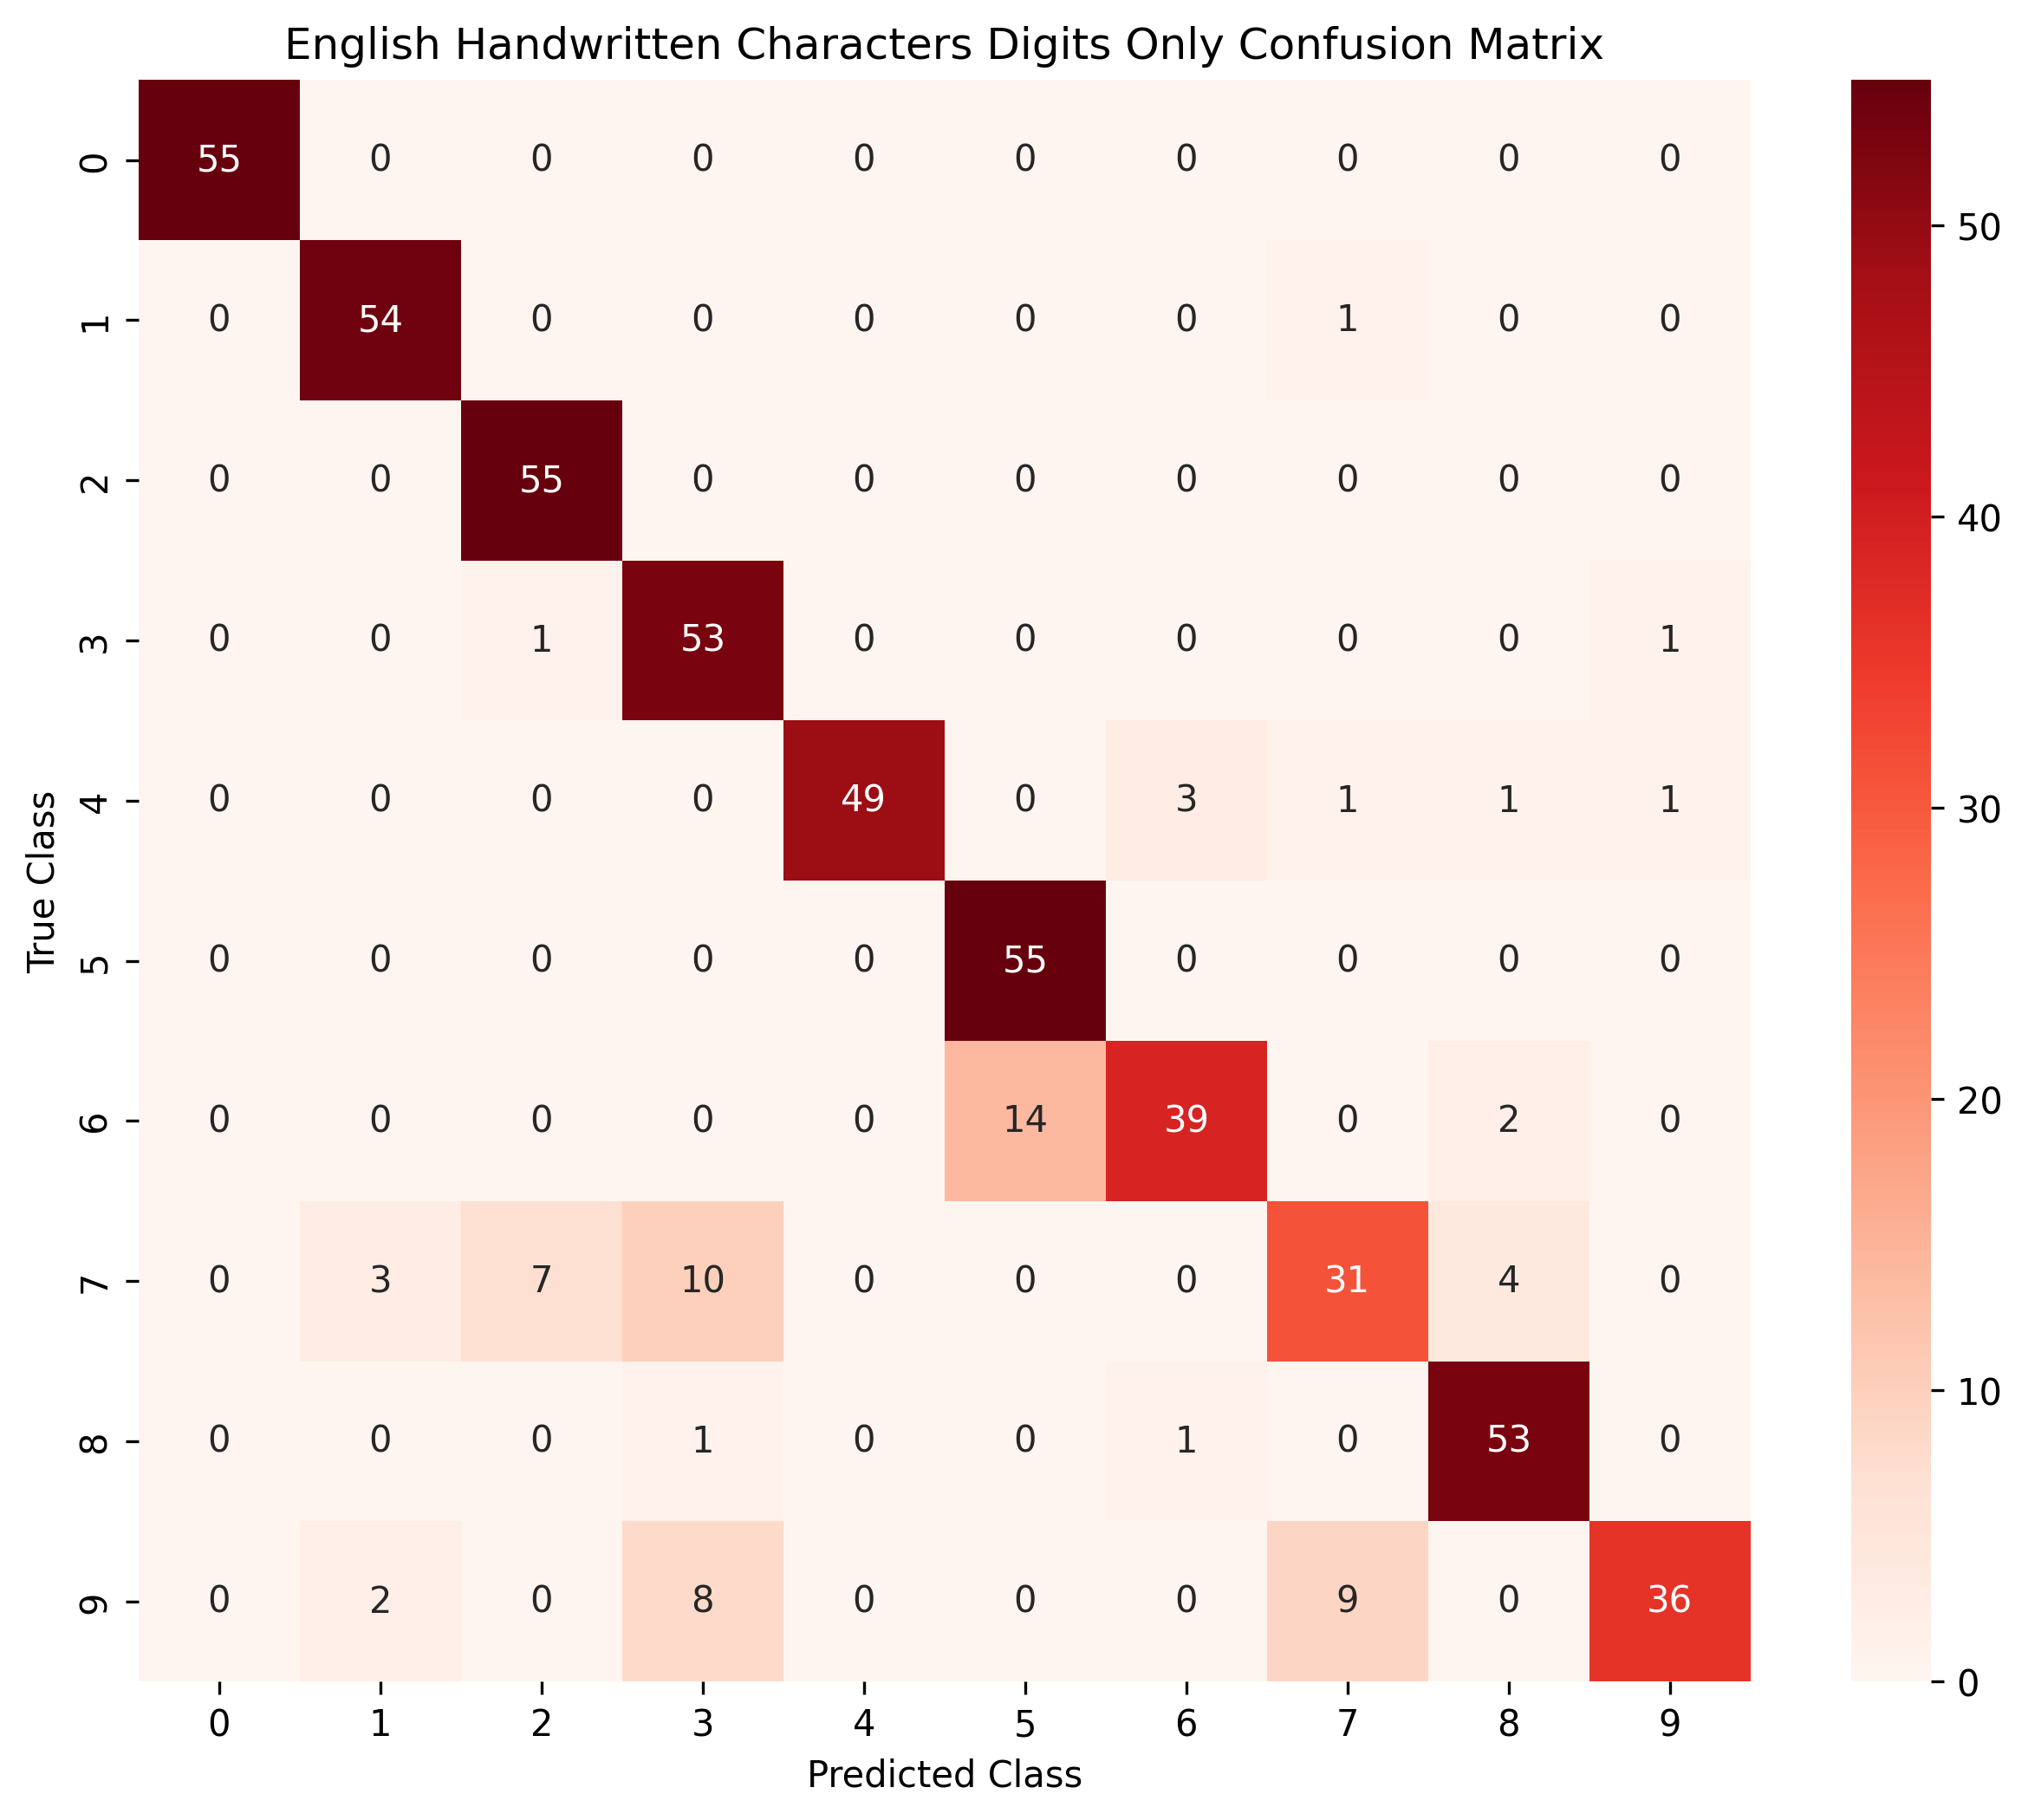
\includegraphics[width=0.99\columnwidth]{Figures/Results/HandwrittenCharacters/english_handwritten_characters_digits_only_confusion_matrix.png}
    \caption{English Handwritten Characters (digits only) confusion matrix for 550 predictions}
\label{fig:english_handwritten_characters_digits_only_confusion_matrix}
\end{figure}


% Digit 0: Number of alphabetic characters predicted as this digit: 528
% Digit 0: Minimum distance: 0.0016648656067618573
% Digit 0: Average distance: 0.16058877589020398
% Digit 0: Original index of the alphabetic character with min distance: 675
% Digit 0: Closest alphabetic character is 'C' (class 12)
% Digit 1: Number of alphabetic characters predicted as this digit: 365
% Digit 1: Minimum distance: 0.003745016885533488
% Digit 1: Average distance: 0.22722867838585623
% Digit 1: Original index of the alphabetic character with min distance: 3082
% Digit 1: Closest alphabetic character is 'u' (class 56)
% Digit 2: Number of alphabetic characters predicted as this digit: 242
% Digit 2: Minimum distance: 0.008925071596907863
% Digit 2: Average distance: 0.20964367917220236
% Digit 2: Original index of the alphabetic character with min distance: 3403
% Digit 2: Closest alphabetic character is 'z' (class 61)
% Digit 3: Number of alphabetic characters predicted as this digit: 85
% Digit 3: Minimum distance: 0.010936401745817276
% Digit 3: Average distance: 0.36543237233574044
% Digit 3: Original index of the alphabetic character with min distance: 1056
% Digit 3: Closest alphabetic character is 'J' (class 19)
% Digit 4: Number of alphabetic characters predicted as this digit: 493
% Digit 4: Minimum distance: 0.005890099717802539
% Digit 4: Average distance: 0.14786566703699247
% Digit 4: Original index of the alphabetic character with min distance: 568
% Digit 4: Closest alphabetic character is 'A' (class 10)


% ALphabetic characters distance to centroids
% alpha_thresholds, alpha_indexes, alpha_avg_distances = find_thresholds_alphabetic_only(data_np)

% plot_alphabetic_distances(alpha_thresholds, alpha_avg_distances, prefix="English Handwritten Alphabetic Characters ", filename="english_handwritten_characters_alphabetic_only_thresholds", save=True)
% # Saved as english_handwritten_characters_alphabetic_only_thresholds.png

\begin{figure}[ht]
    \centering
    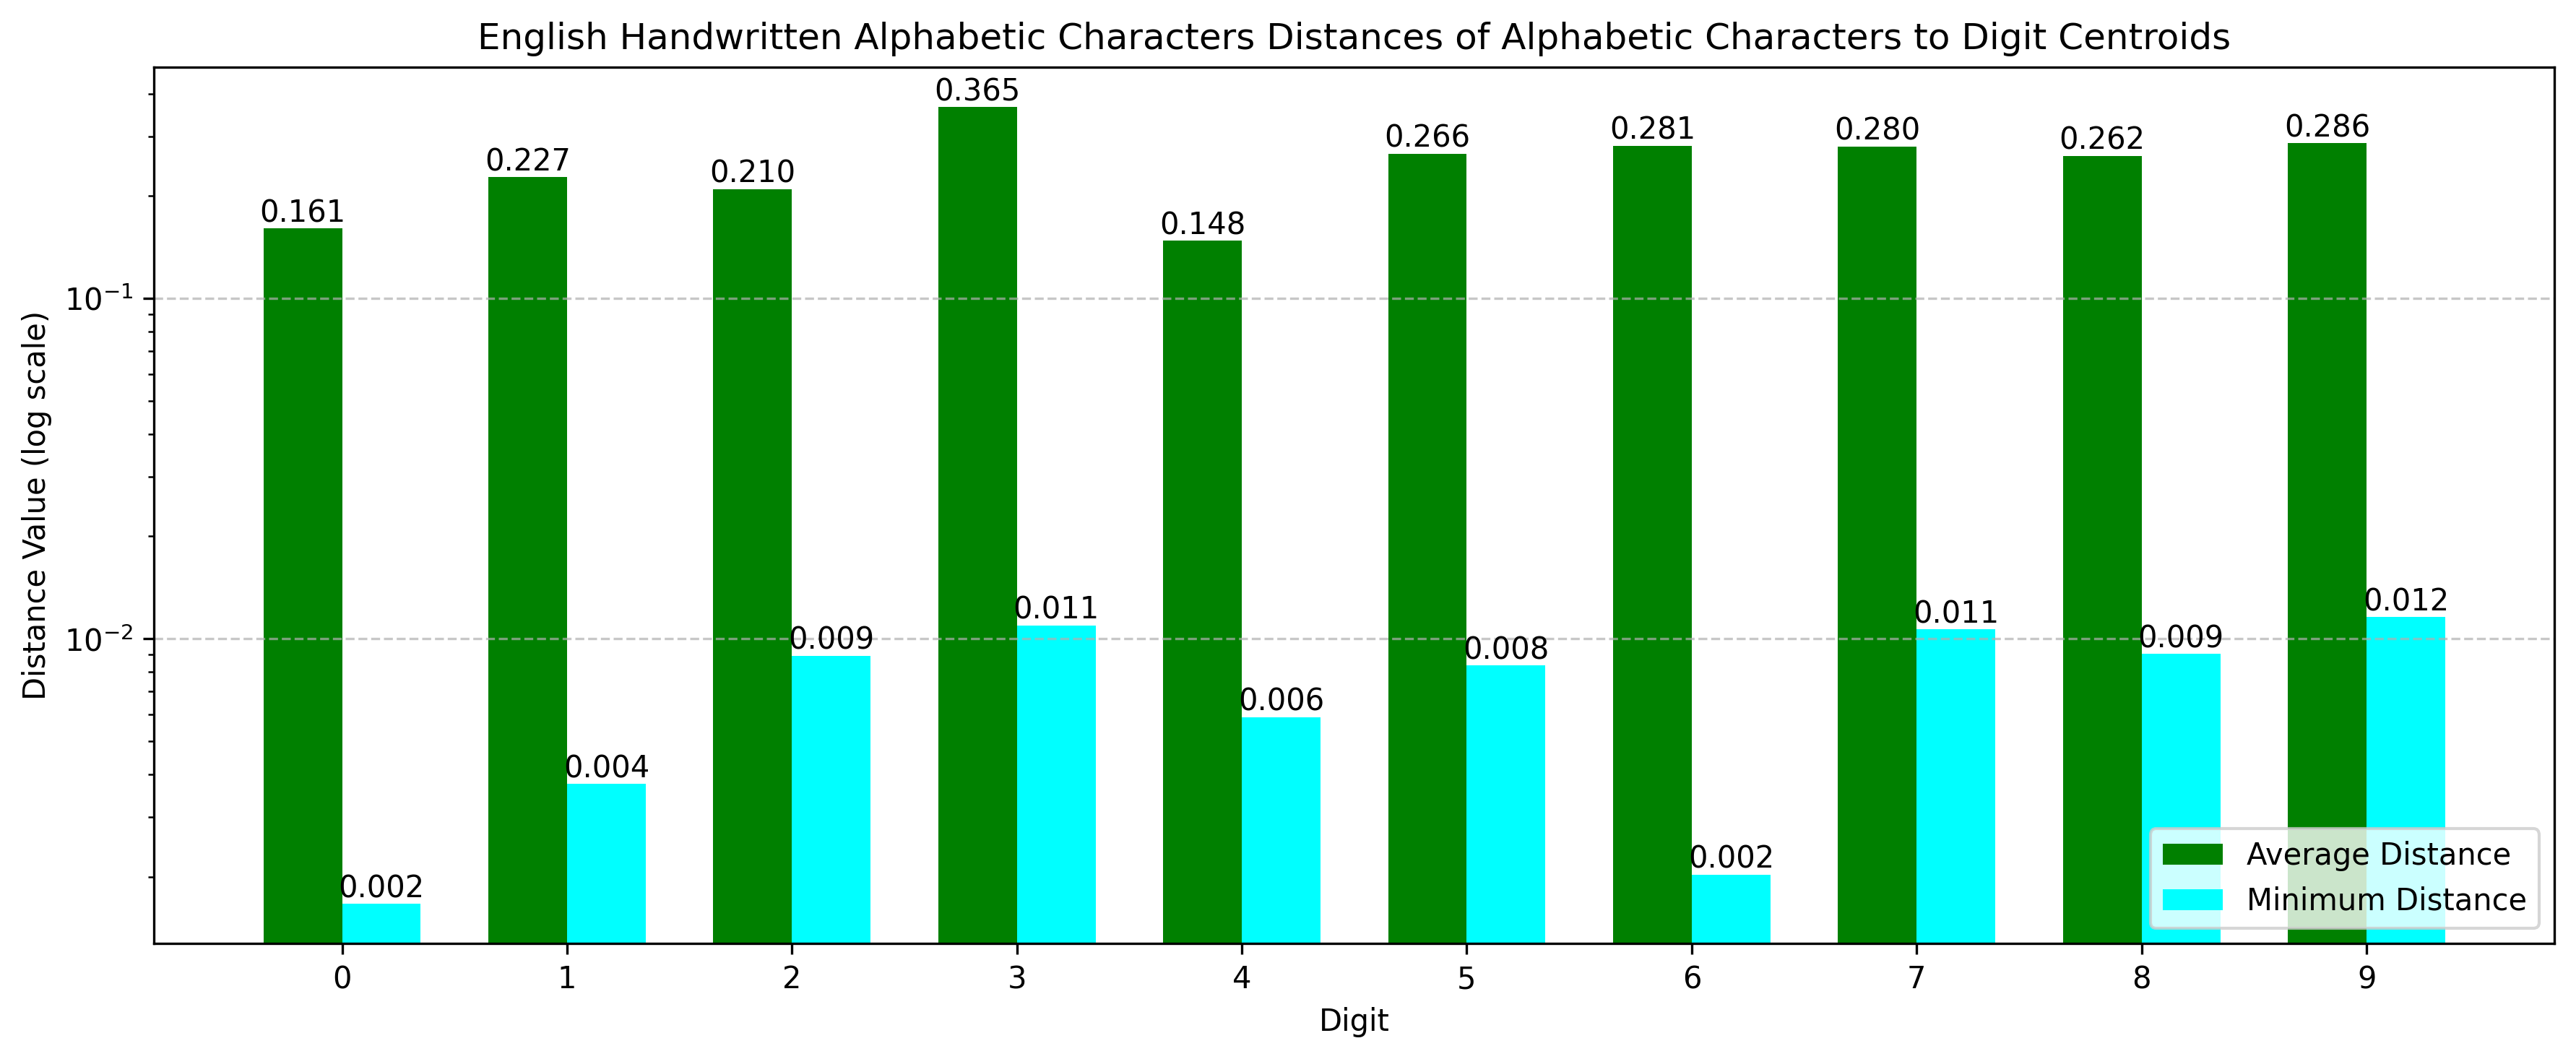
\includegraphics[width=0.99\columnwidth]{Figures/Results/HandwrittenCharacters/english_handwritten_characters_alphabetic_only_thresholds.png}
    \caption{English Handwritten Alphabetic Characters average and minimum distances to digit class centroids, where all examples have are "misclassified" given network was trained on digits only}
\label{fig:english_handwritten_characters_alphabetic_only_thresholds}
\end{figure}

% \begin{sidewaystable}[h]
% \centering
% \caption{Alphabetic Character Prediction Threshold Table}
% \begin{tabular}{c *{10}{S[table-format=3.0]@{\ (\si{\percent})}}
%                 S[table-format=4.0]@{\ (\si{\percent})} 
%                 S[table-format=4.0]@{\ (\si{\percent})}}
% \toprule
% {Thresh} & {0 (\%)} & {1 (\%)} & {2 (\%)} & {3 (\%)} & {4 (\%)} & {5 (\%)} & {6 (\%)} & {7 (\%)} & {8 (\%)} & {9 (\%)} & {TBT (\%)} & {TAT (\%)} \\
% \midrule
% 0.80 & 528 & 365 & 242 & 85 & 493 & 239 & 223 & 108 & 517 & 60 & 2860 & 0 \\ % Totals row, TAT = 0%
% 0.70 & 518 {(\SI{98.1}{\percent})} & 359 {(\SI{98.4}{\percent})} & 236 {(\SI{97.5}{\percent})} & 81 {(\SI{95.3}{\percent})} & 481 {(\SI{97.6}{\percent})} & 229 {(\SI{95.8}{\percent})} & 212 {(\SI{95.1}{\percent})} & 104 {(\SI{96.3}{\percent})} & 508 {(\SI{98.3}{\percent})} & 58 {(\SI{96.7}{\percent})} & 2786 {(\SI{97.4}{\percent})} & 74 {(\SI{2.6}{\percent})} \\
% 0.60 & 497 {(\SI{94.1}{\percent})} & 333 {(\SI{91.2}{\percent})} & 217 {(\SI{89.7}{\percent})} & 68 {(\SI{80.0}{\percent})} & 461 {(\SI{93.5}{\percent})} & 205 {(\SI{85.8}{\percent})} & 195 {(\SI{87.4}{\percent})} & 93 {(\SI{86.1}{\percent})} & 459 {(\SI{88.8}{\percent})} & 51 {(\SI{85.0}{\percent})} & 2579 {(\SI{90.2}{\percent})} & 281 {(\SI{9.8}{\percent})} \\
% 0.50 & 470 {(\SI{89.0}{\percent})} & 304 {(\SI{83.3}{\percent})} & 201 {(\SI{83.1}{\percent})} & 52 {(\SI{61.2}{\percent})} & 440 {(\SI{89.2}{\percent})} & 184 {(\SI{77.0}{\percent})} & 174 {(\SI{78.0}{\percent})} & 87 {(\SI{80.6}{\percent})} & 414 {(\SI{80.1}{\percent})} & 47 {(\SI{78.3}{\percent})} & 2373 {(\SI{83.0}{\percent})} & 487 {(\SI{17.0}{\percent})} \\
% 0.40 & 442 {(\SI{83.7}{\percent})} & 272 {(\SI{74.5}{\percent})} & 181 {(\SI{74.8}{\percent})} & 44 {(\SI{51.8}{\percent})} & 420 {(\SI{85.2}{\percent})} & 157 {(\SI{65.7}{\percent})} & 153 {(\SI{68.6}{\percent})} & 75 {(\SI{69.4}{\percent})} & 365 {(\SI{70.6}{\percent})} & 37 {(\SI{61.7}{\percent})} & 2146 {(\SI{75.0}{\percent})} & 714 {(\SI{25.0}{\percent})} \\
% 0.30 & 407 {(\SI{77.1}{\percent})} & 238 {(\SI{65.2}{\percent})} & 167 {(\SI{69.0}{\percent})} & 38 {(\SI{44.7}{\percent})} & 397 {(\SI{80.5}{\percent})} & 141 {(\SI{59.0}{\percent})} & 124 {(\SI{55.6}{\percent})} & 61 {(\SI{56.5}{\percent})} & 317 {(\SI{61.3}{\percent})} & 33 {(\SI{55.0}{\percent})} & 1923 {(\SI{67.2}{\percent})} & 937 {(\SI{32.8}{\percent})} \\
% 0.20 & 365 {(\SI{69.1}{\percent})} & 206 {(\SI{56.4}{\percent})} & 147 {(\SI{60.7}{\percent})} & 25 {(\SI{29.4}{\percent})} & 368 {(\SI{74.6}{\percent})} & 122 {(\SI{51.0}{\percent})} & 98 {(\SI{43.9}{\percent})} & 48 {(\SI{44.4}{\percent})} & 253 {(\SI{48.9}{\percent})} & 27 {(\SI{45.0}{\percent})} & 1659 {(\SI{58.0}{\percent})} & 1201 {(\SI{42.0}{\percent})} \\
% 0.10 & 320 {(\SI{60.6}{\percent})} & 154 {(\SI{42.2}{\percent})} & 127 {(\SI{52.5}{\percent})} & 16 {(\SI{18.8}{\percent})} & 314 {(\SI{63.7}{\percent})} & 100 {(\SI{41.8}{\percent})} & 76 {(\SI{34.1}{\percent})} & 32 {(\SI{29.6}{\percent})} & 183 {(\SI{35.4}{\percent})} & 22 {(\SI{36.7}{\percent})} & 1344 {(\SI{47.0}{\percent})} & 1516 {(\SI{53.0}{\percent})} \\
% 0.05 & 272 {(\SI{51.5}{\percent})} & 125 {(\SI{34.2}{\percent})} & 111 {(\SI{45.9}{\percent})} & 10 {(\SI{11.8}{\percent})} & 274 {(\SI{55.6}{\percent})} & 77 {(\SI{32.2}{\percent})} & 57 {(\SI{25.6}{\percent})} & 22 {(\SI{20.4}{\percent})} & 140 {(\SI{27.1}{\percent})} & 18 {(\SI{30.0}{\percent})} & 1106 {(\SI{38.7}{\percent})} & 1754 {(\SI{61.3}{\percent})} \\
% 0.02 & 228 {(\SI{43.2}{\percent})} & 101 {(\SI{27.7}{\percent})} & 71 {(\SI{29.3}{\percent})} & 8 {(\SI{9.4}{\percent})} & 240 {(\SI{48.7}{\percent})} & 56 {(\SI{23.4}{\percent})} & 30 {(\SI{13.5}{\percent})} & 18 {(\SI{16.7}{\percent})} & 12 {(\SI{2.3}{\percent})} & 10 {(\SI{16.7}{\percent})} & 774 {(\SI{27.1}{\percent})} & 2086 {(\SI{72.9}{\percent})} \\
% \bottomrule
% \end{tabular}
% \end{sidewaystable}

% data from
%np.save('data/grok_0.8_0.02_alphabetic_prediction_thresholds.npy', alpha_threshold_table)

\begin{table}[ht]
\centering
\caption{Alphabetic Character Prediction Threshold Table: Percentages (top) and Numeric Values (bottom)}
\label{tab:combined}
\scriptsize
\begin{tabular}{lccccccccccccc}
\toprule
\multicolumn{13}{c}{\textbf{Percentages (relative to baseline at 0.80)}} \\
\midrule
Thresh & 0 (\%) & 1 (\%) & 2 (\%) & 3 (\%) & 4 (\%) & 5 (\%) & 6 (\%) & 7 (\%) & 8 (\%) & 9 (\%) & TBT (\%) & TAT (\%) \\
\midrule
0.80   & 100.0  & 100.0  & 100.0  & 100.0  & 100.0  & 100.0  & 100.0  & 100.0  & 100.0  & 100.0  & 100.0   & 0.0   \\
0.70   & 98.1   & 98.2   & 97.5   & 95.3   & 97.5   & 95.8   & 95.2   & 96.3   & 98.1   & 96.7   & 97.4    & 2.6   \\
0.60   & 94.2   & 91.2   & 89.7   & 80.0   & 93.5   & 85.8   & 87.5   & 86.1   & 88.8   & 85.0   & 90.2    & 9.8   \\
0.50   & 89.0   & 83.3   & 83.1   & 61.2   & 89.2   & 77.0   & 78.0   & 80.6   & 80.0   & 78.3   & 82.9    & 17.1  \\
0.40   & 83.7   & 74.5   & 74.8   & 51.8   & 85.3   & 65.6   & 68.6   & 69.4   & 70.6   & 61.7   & 75.0    & 25.0  \\
0.30   & 77.1   & 65.2   & 69.0   & 44.7   & 80.6   & 58.9   & 55.6   & 56.5   & 61.3   & 55.0   & 67.2    & 32.8  \\
0.20   & 69.2   & 56.4   & 60.7   & 29.4   & 74.7   & 51.1   & 44.0   & 44.4   & 48.9   & 45.0   & 58.0    & 42.0  \\
0.10   & 60.6   & 42.2   & 52.5   & 18.8   & 63.8   & 41.8   & 34.1   & 29.6   & 35.4   & 36.7   & 47.1    & 52.9  \\
0.05   & 51.5   & 34.3   & 45.9   & 11.8   & 55.6   & 32.2   & 25.6   & 20.4   & 27.1   & 30.0   & 38.7    & 61.3  \\
0.02   & 43.2   & 27.7   & 29.4   & 9.4    & 48.7   & 23.4   & 13.5   & 16.7   & 2.3    & 16.7   & 27.1    & 72.9  \\
\midrule
\multicolumn{13}{c}{\textbf{Numeric Values}} \\
\midrule
Thresh & 0 & 1 & 2 & 3 & 4 & 5 & 6 & 7 & 8 & 9 & TBT & TAT \\
\midrule
0.80   & 528 & 365 & 242 & 85  & 493 & 239 & 223 & 108 & 517 & 60  & 2860 & 0   \\
0.70   & 518 & 359 & 236 & 81  & 481 & 229 & 212 & 104 & 508 & 58  & 2786 & 74  \\
0.60   & 497 & 333 & 217 & 68  & 461 & 205 & 195 & 93  & 459 & 51  & 2579 & 281 \\
0.50   & 470 & 304 & 201 & 52  & 440 & 184 & 174 & 87  & 414 & 47  & 2373 & 487 \\
0.40   & 442 & 272 & 181 & 44  & 420 & 157 & 153 & 75  & 365 & 37  & 2146 & 714 \\
0.30   & 407 & 238 & 167 & 38  & 397 & 141 & 124 & 61  & 317 & 33  & 1923 & 937 \\
0.20   & 365 & 206 & 147 & 25  & 368 & 122 & 98  & 48  & 253 & 27  & 1659 & 1201\\
0.10   & 320 & 154 & 127 & 16  & 314 & 100 & 76  & 32  & 183 & 22  & 1344 & 1516\\
0.05   & 272 & 125 & 111 & 10  & 274 & 77  & 57  & 22  & 140 & 18  & 1106 & 1754\\
0.02   & 228 & 101 & 71  & 8   & 240 & 56  & 30  & 18  & 12  & 10  & 774  & 2086\\
\bottomrule
\end{tabular}
\label{app:alphabetic_mnist_cnn_misclassifications}
\end{table}

Table \ref{app:alphabetic_mnist_cnn_misclassifications} displays data from the MNIST CNN classifier applied to alphabetic characters from the English Handwritten Character dataset. Note all classifications are incorrect because there is no true class for alphabetic characters. The upper table shows percentages calculated relative to the total examples baseline row at threshold 0.80. In the baseline, each digit column and TBT (Total below threshold) are 100.0\%, i.e. all examples are below threshold and TAT (total above threshold is 0.0\% i.e. no examples are above threshold, meaning no examples are classed as "don't know". In the following rows, the percentages for digit columns and TBT decrease as the threshold value decreases, while the percentage for TAT increases correspondingly, as more examples are set to "don't know". The aim is to set the threshold at a level that would exclude the maximum number of alphabetic characters, while still making the model usable.

The lower table presents the corresponding raw counts. At threshold 0.80, the digit counts sum to 2860 with TAT equal to 0. As the threshold value is reduced, the counts in each digit column decrease. Simultaneously, the value for TBT declines and the count for TAT increases. The change in values is consistent across all digit columns. The two tables together provide both normalized and absolute perspectives on the distribution of predictions as a function of the distance threshold.

The baseline row contains counts of 528, 365, 242, 85, 493, 239, 223, 108, 517, and 60 for digits 0 through 9, respectively. Counts in columns 0, 4, and 8 record 528, 493, and 517, while counts in columns 3, 7, and 9 record 85, 108, and 60. These values indicate that misclassifications resulting in digits 0, 4, and 8 occur in a greater number of instances than those resulting in digits 3, 7, and 9.

The impact of having unknown data can be assessed by referencing table \ref{app:enhanced_threshold_analysis}, where at a threshold of 0.05 the accuracy on the remaining data (91\%) is close to 100\%), corresponding to approximately 55k examples. The number of alphabetic characters where the softmax output is still below threshold is about 1k, so given the proportions, it would impact the accuracy in the single digit order of magnitude, and also decrease the ratio of correct / incorrect predictions up to threshold.

\begin{table*}[ht]
\centering
\tiny
\caption{Enhanced Threshold Analysis with Meta Metrics. 
Please zoom in for details. Key columns:
\textbf{Thresh}: Class threshold;
\textbf{Ret\%}: Retention percentage;
\textbf{Acc\%}: Accuracy percentage;
\textbf{Corr}: Correct predictions retained;
\textbf{Incor}: Incorrect predictions retained;
\textbf{CLost}: Cumulative correct lost;
\textbf{CElim}: Cumulative incorrect eliminated;
\textbf{Ratio}: Correct:Incorrect ratio;
\textbf{MetaT}: Meta threshold;
\textbf{PtsIn}: Points inside meta hypersphere;
\textbf{NoCls}: Points outside both class and meta hyperspheres;
\textbf{\%CLst}: Percentage of total correct lost;
\textbf{\%CEm}: Percentage of total incorrect eliminated;
\textbf{\%Pts}: Percentage of dataset inside meta hypersphere;
\textbf{\%NCl}: Percentage of dataset in no-class zone.}
\label{tab:threshold_analysis}
\begin{tabular}{r r r r r r r r r r r r r r r r}
\toprule
Thresh & Ret\% & Acc\% & Corr & Incor & CLost & CElim & Ratio & MetaT & PtsIn & NoCls & \%CLst & \%CEm & \%Pts & \%NCl \\
\midrule
0.80 & 100.00\% & 98.46\% & 59073 & 926 & 1 & 0 & 64:1 & 0.1337 & 0 & 1 & 0.0017\% & 0.00\% & 0.00\% & 0.0017\% \\
0.70 & 99.87\% & 98.54\% & 59048 & 876 & 26 & 50 & 67:1 & 0.2337 & 0 & 76 & 0.0440\% & 5.40\% & 0.00\% & 0.1267\% \\
0.60 & 99.27\% & 98.83\% & 58863 & 699 & 211 & 227 & 84:1 & 0.3337 & 5 & 433 & 0.3572\% & 24.51\% & 0.01\% & 0.7217\% \\
0.50 & 98.66\% & 99.04\% & 58626 & 568 & 448 & 358 & 103:1 & 0.4337 & 60 & 746 & 0.7584\% & 38.66\% & 0.10\% & 1.2433\% \\
0.40 & 98.00\% & 99.25\% & 58355 & 442 & 719 & 484 & 132:1 & 0.5337 & 274 & 929 & 1.2171\% & 52.27\% & 0.46\% & 1.5483\% \\
0.30 & 97.20\% & 99.42\% & 57981 & 338 & 1093 & 588 & 172:1 & 0.6337 & 889 & 792 & 1.8502\% & 63.50\% & 1.48\% & 1.3200\% \\
0.20 & 96.09\% & 99.58\% & 57411 & 242 & 1663 & 684 & 237:1 & 0.7337 & 1830 & 517 & 2.8151\% & 73.87\% & 3.05\% & 0.8617\% \\
0.10 & 93.92\% & 99.76\% & 56219 & 133 & 2855 & 793 & 423:1 & 0.8337 & 3214 & 434 & 4.8329\% & 85.64\% & 5.36\% & 0.7233\% \\
0.05 & 91.76\% & 99.84\% & 54969 & 87 & 4105 & 839 & 632:1 & 0.8837 & 4904 & 40 & 6.9489\% & 90.60\% & 8.17\% & 0.0667\% \\
\bottomrule
\end{tabular}
\label{app:enhanced_threshold_analysis}
\end{table*}

%%%%%%%%%%%%%%%%%%%%%%%%%%%%%%%%%%%%%%%%%%%%%%%%%%%
% ALPHABETIC x NUMERIC MISCLASSIFICATION HEATMAPS %
%%%%%%%%%%%%%%%%%%%%%%%%%%%%%%%%%%%%%%%%%%%%%%%%%%%

%create_and_save_heatmaps(data_np, filename="figures/english_handwritten_characters_x_confusion_matrix.png", save=True)

Examining the confusion matrices in Figure \ref {fig:english_handwritten_characters_x_confusion_matrix} for uppercase (left) and lowercase (right) alphabetic characters misclassified by the CNN originally trained on MNIST digits reveals several consistent patterns. In particular, letters that share strong visual similarity with digits are frequently misclassified. For instance, uppercase “O” is often misread as “0,” while uppercase “I” may be confused with “1.” Similar issues arise with lowercase letters: “o” tends to be classified as “0,” and “l” can be mistaken for “1.” These trends underscore the model’s reliance on shape-based cues that were reinforced during digit-focused training on MNIST.

The heatmaps show distinct “hotspots” where misclassifications are concentrated, such as uppercase “S” confused with “5” and uppercase “Z” confused with “2.” Lowercase characters with loops and ascenders (e.g., “g,” “q,” “y”) also tend to be misclassified as 9 or other digits containing loops. 

% Plot generated by
\begin{figure}[ht]
    \centering
    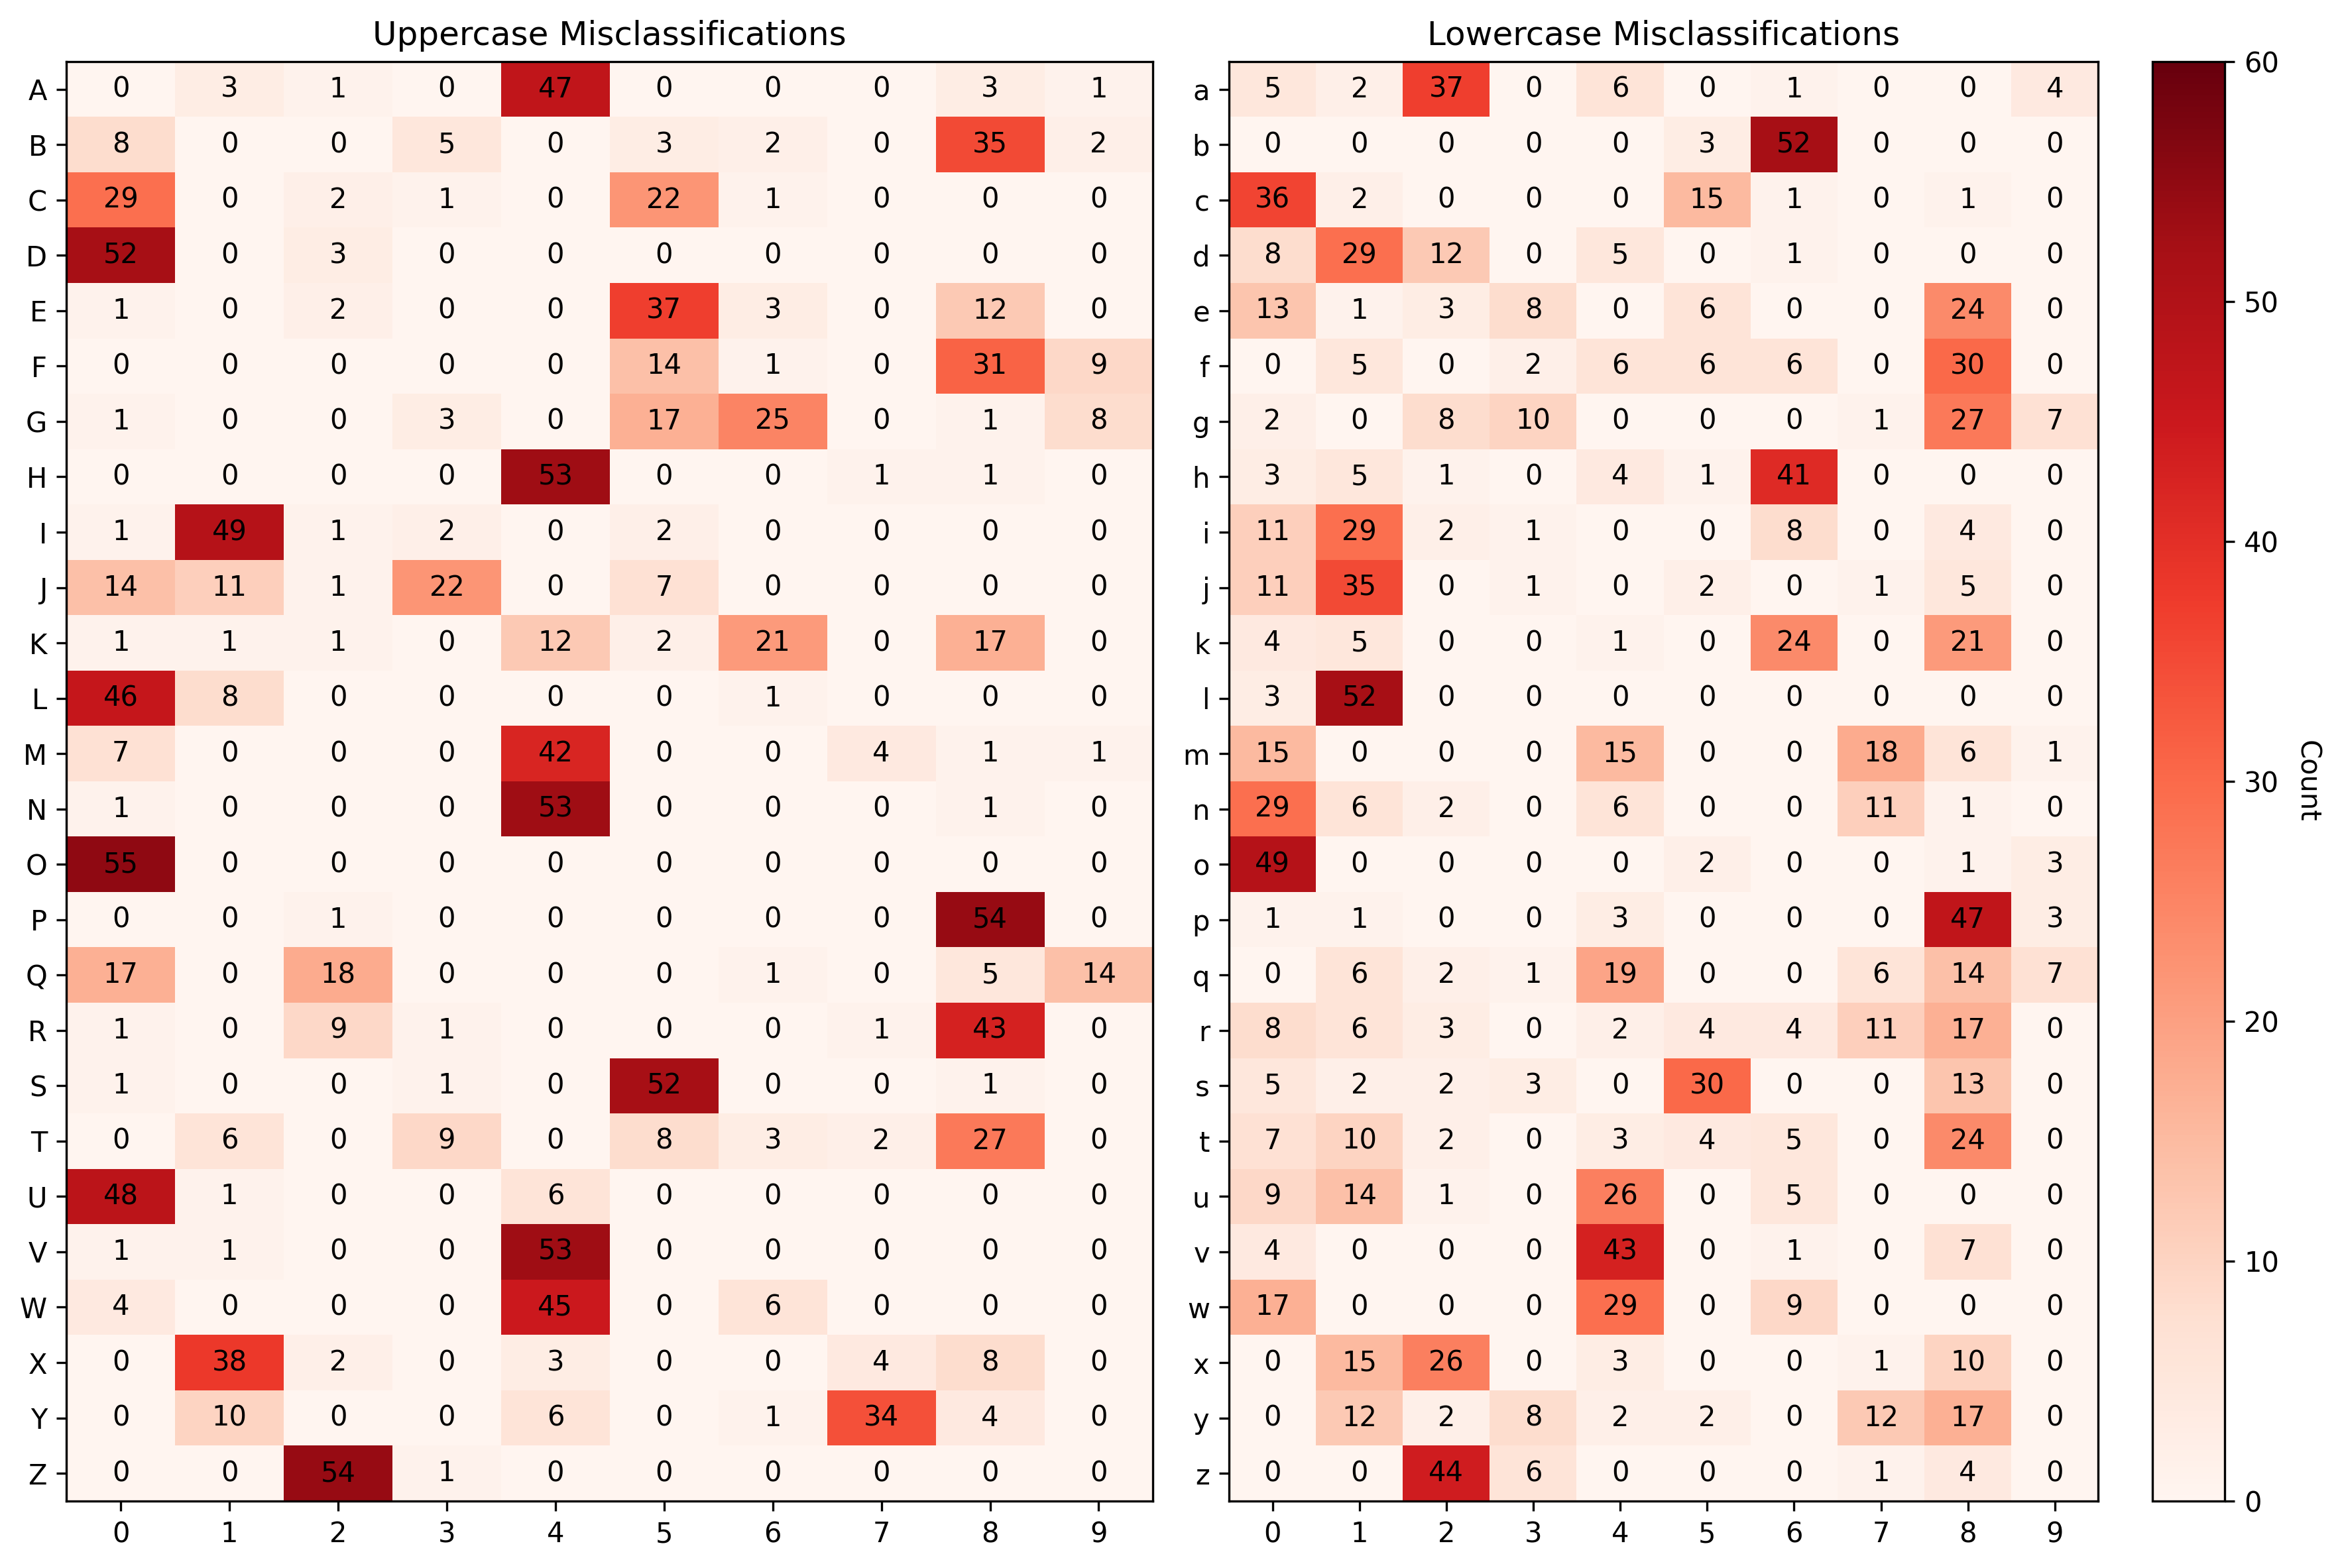
\includegraphics[width=0.99\columnwidth]{Figures/Results/HandwrittenCharacters/english_handwritten_characters_x_confusion_matrix.png}
    \caption{English Handwritten Alphabetic Characters nearest distance and example, and averages}
\label{fig:english_handwritten_characters_x_confusion_matrix}
\end{figure}

%%%%%%%%%%%%%%%%%%%%%%%%%%%%%
% SOFTMAX OUTPUT COMPARISON %
%%%%%%%%%%%%%%%%%%%%%%%%%%%%%

% function call (work in progress repo)
% plot_digit_averages(test_correct_predictions, test_incorrect_predictions, color1='lightgreen', color2='lightcoral', data="Testing Data")

% Figure \ref{fig:MNIST_Softmax_Averages_Training_appendix} shows the softmax output for correctly and incorrectly classified digits from the MNIST training dataset (60k examples) while Figure \ref{fig:english_handwritten_characters_digit_softmax_averages} shows the softmax output for correctly and incorrectly digits (alphabetic characters excluded) classifications of the English Handwritten Character MNISTified dataset (550 examples) no "0" or "4" digits where misclassified, hence the blank plots in the second row (misclassifications).
% % Figure \ref{fig:english_handwritten_characters_alphabetic_softmax_averages}

% \begin{figure*}[ht]
%     \centering
%     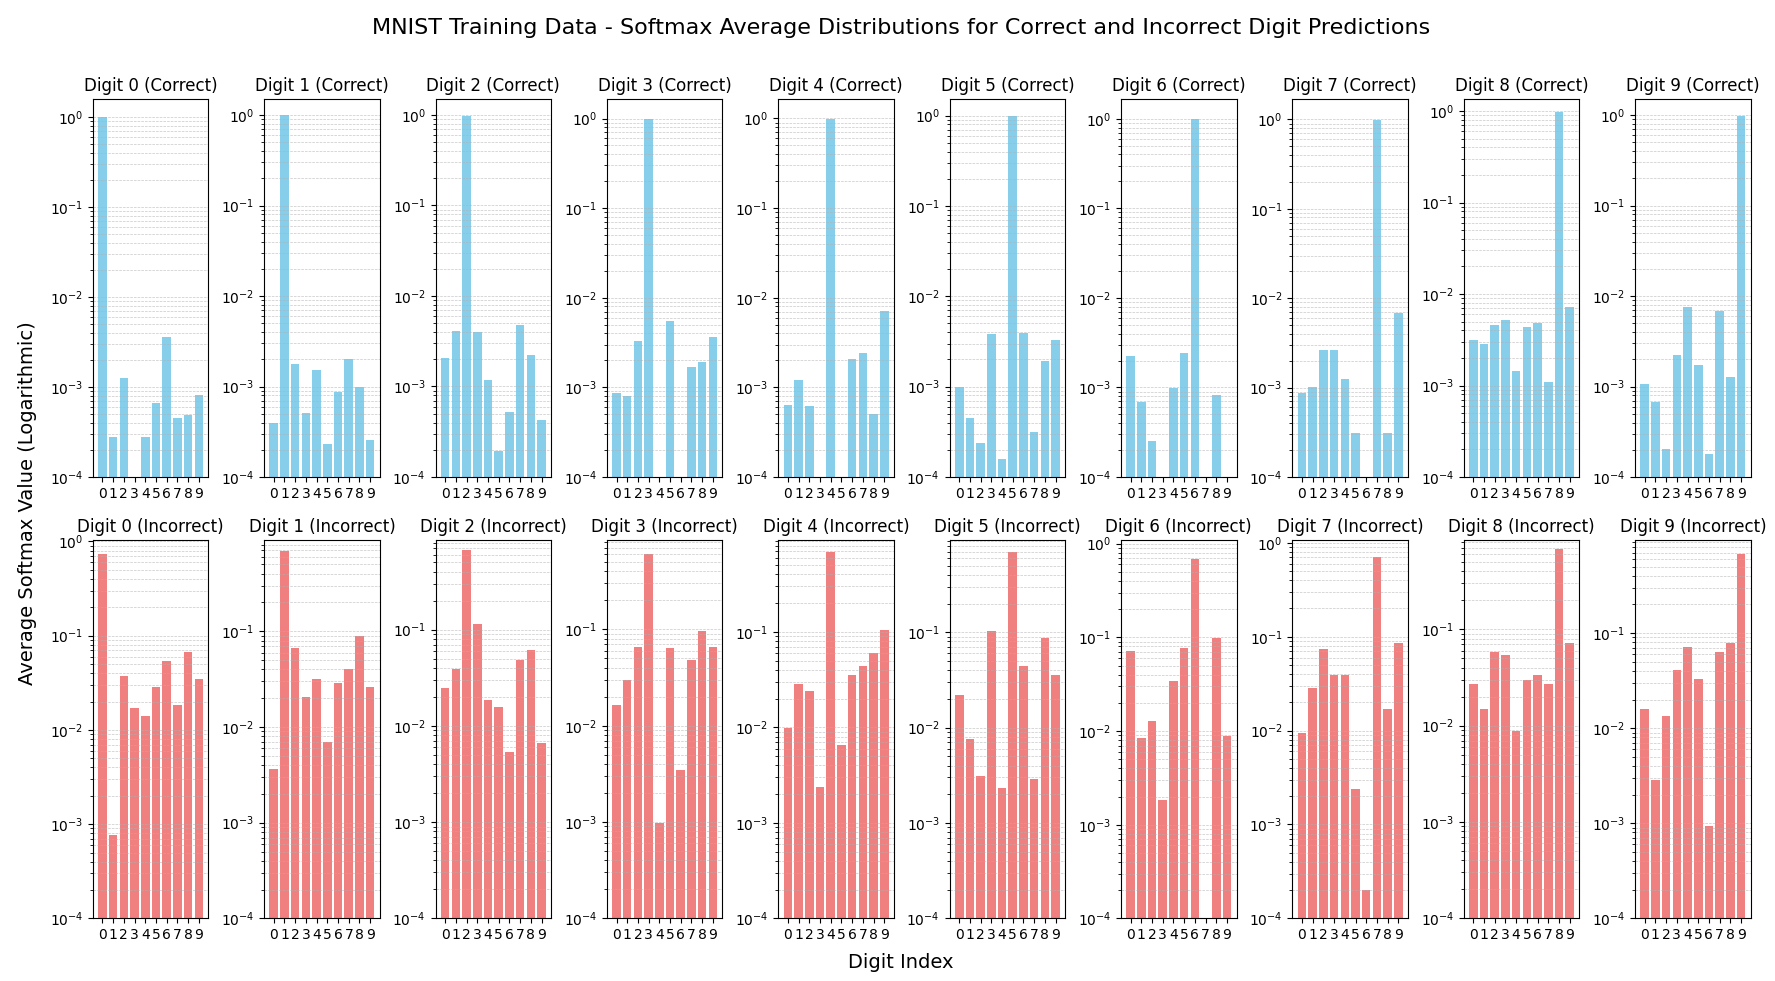
\includegraphics[width=0.99\textwidth]{Figures/Results/HandwrittenCharacters/MNIST_Softmax_Averages_Training.png}
%     \caption{Average Softmax Probabilities for Correctly and Incorrectly Classified Digits in the MNIST Training Dataset.}
%     \label{fig:MNIST_Softmax_Averages_Training_appendix}
% \end{figure*}

% \begin{figure*}[ht]
%     \centering
%     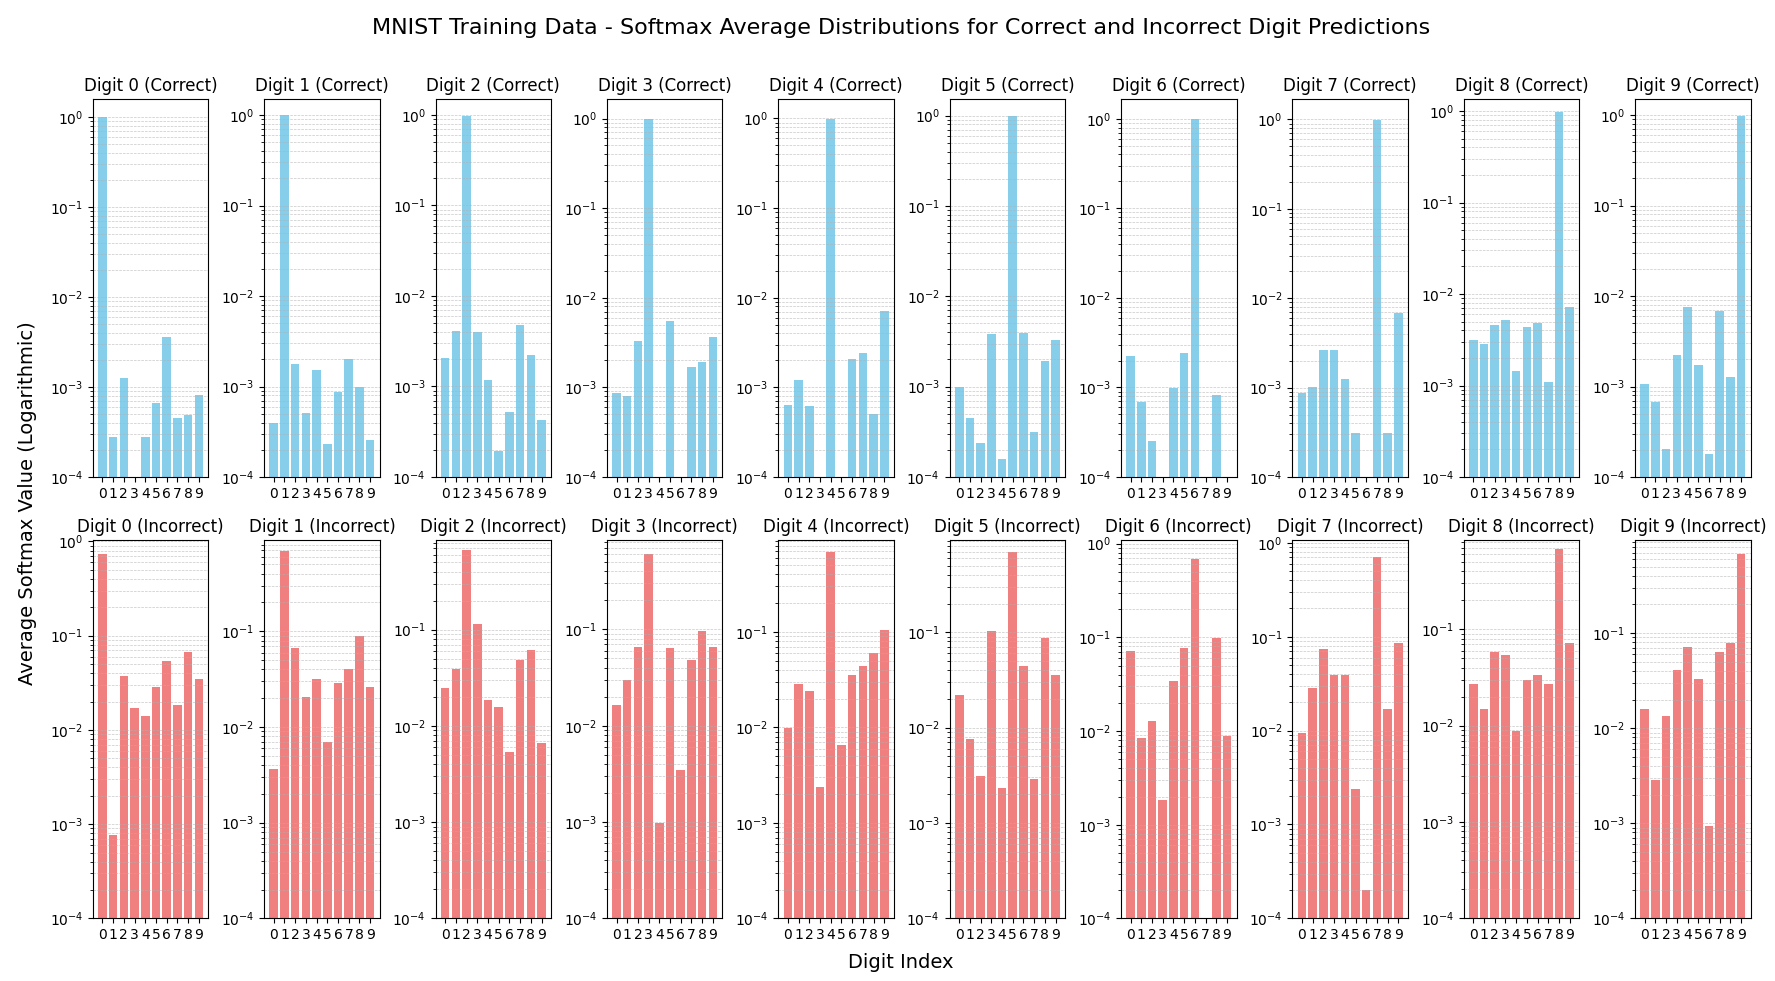
\includegraphics[width=0.99\textwidth]{Figures/Results/HandwrittenCharacters/MNIST_Softmax_Averages_Training.png}
%     \caption{Average Softmax Probabilities for Correctly and Incorrectly Classified Digits in the English Handwritten Characters Dataset (excludes alphabetical character predictions).}
%     \label{fig:english_handwritten_characters_digit_softmax_averages}
% \end{figure*}

% Generated by function call:
% plot_digit_averages(correct_digit_predictions, incorrect_digit_predictions, color1='skyblue', color2='lightcoral', data="English Handwritten Characters Digits Only", title= "Softmax Average Distributions for Correct and Incorrect Digit Predictions", filename="figures/english_handwritten_characters_digit_softmax_averages.png", save=True)
% # Saved average softmax outputs for correct and incorrect digit predictiions. figures/english_handwritten_characters_digit_softmax_averages.png

  
% \begin{figure*}[ht]
%     \centering
%     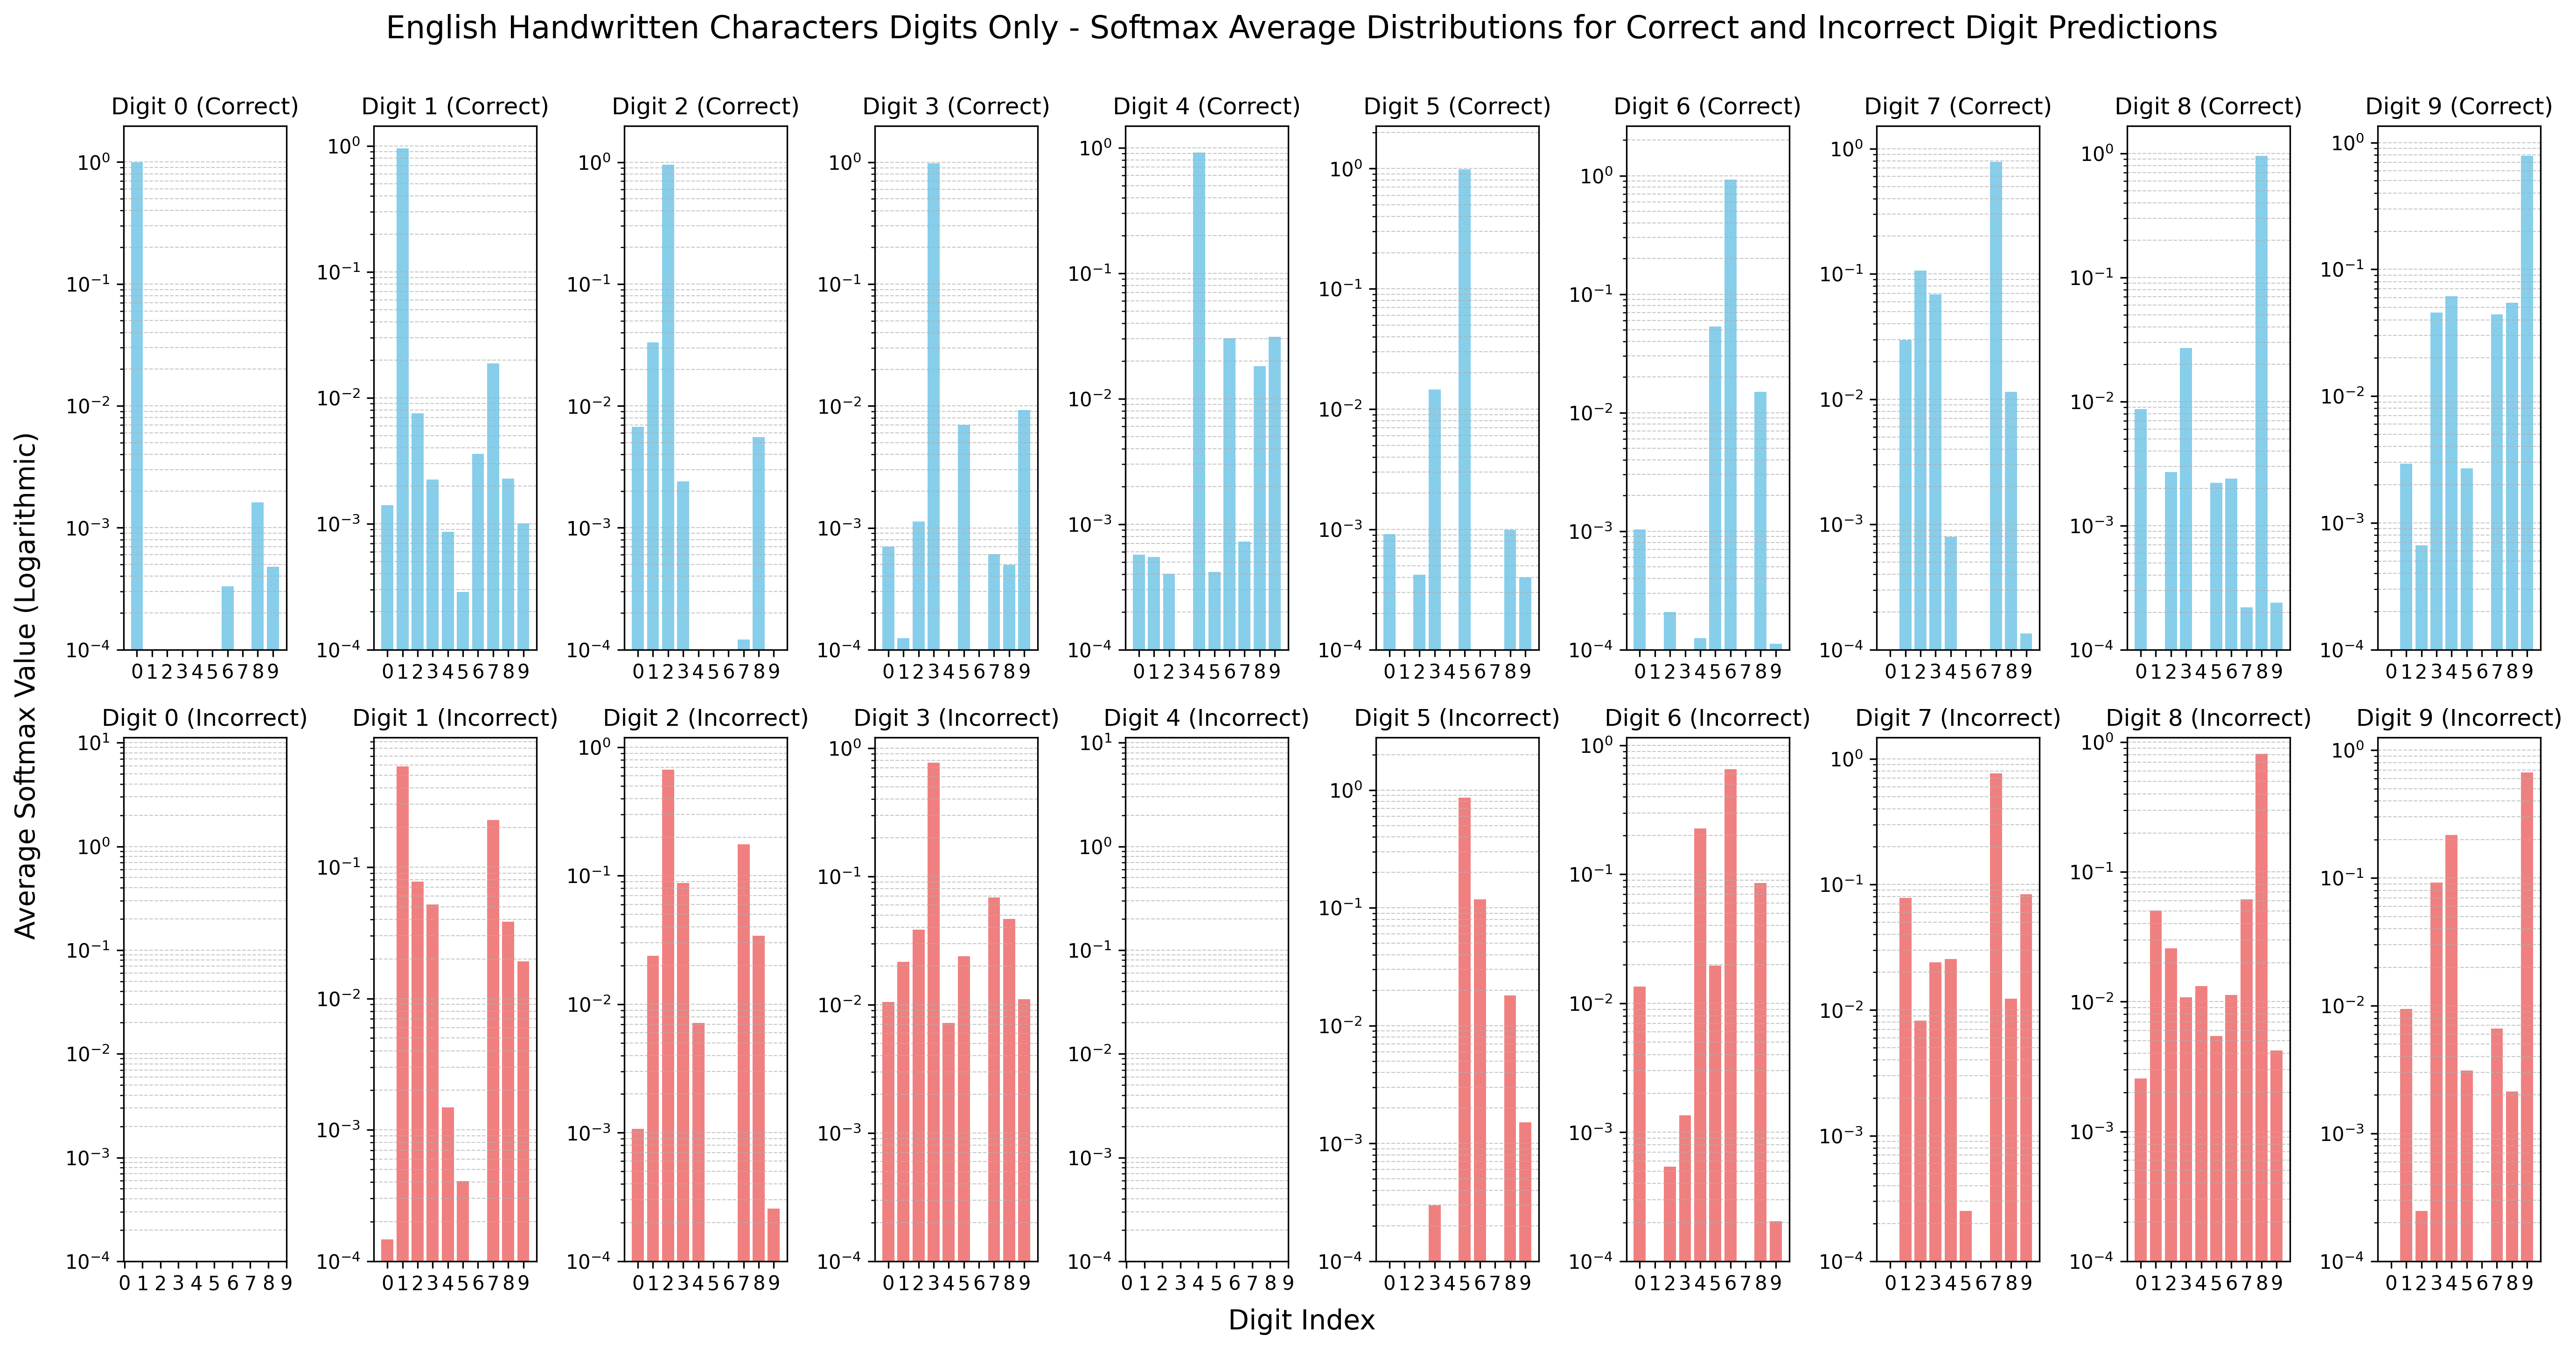
\includegraphics[width=0.99\textwidth]{Figures/Results/HandwrittenCharacters/english_handwritten_characters_digit_softmax_averages.png}
%     \caption{Average Softmax Probabilities for Correctly and Incorrectly Classified Digits in the English Handwritten Character MNISTified Dataset}
% \label{fig:english_handwritten_characters_digit_softmax_averages}
% \end{figure*}

% % plot_alphabetic_character_averages(alphabetic_predictions, color='lightcoral', data="English Handwritten Characters - Alphabetic Only", title="Softmax Average Distributions for Alphabetic Character Predictions", filename="figures/english_handwritten_characters_alphabetic_softmax_averages.png", save=True)
% % # Saved average softmax outputs for incorrect alphabetic character predictions. figures/english_handwritten_characters_alphabetic_softmax_averages.png

% \begin{figure*}[ht]
%     \centering
%     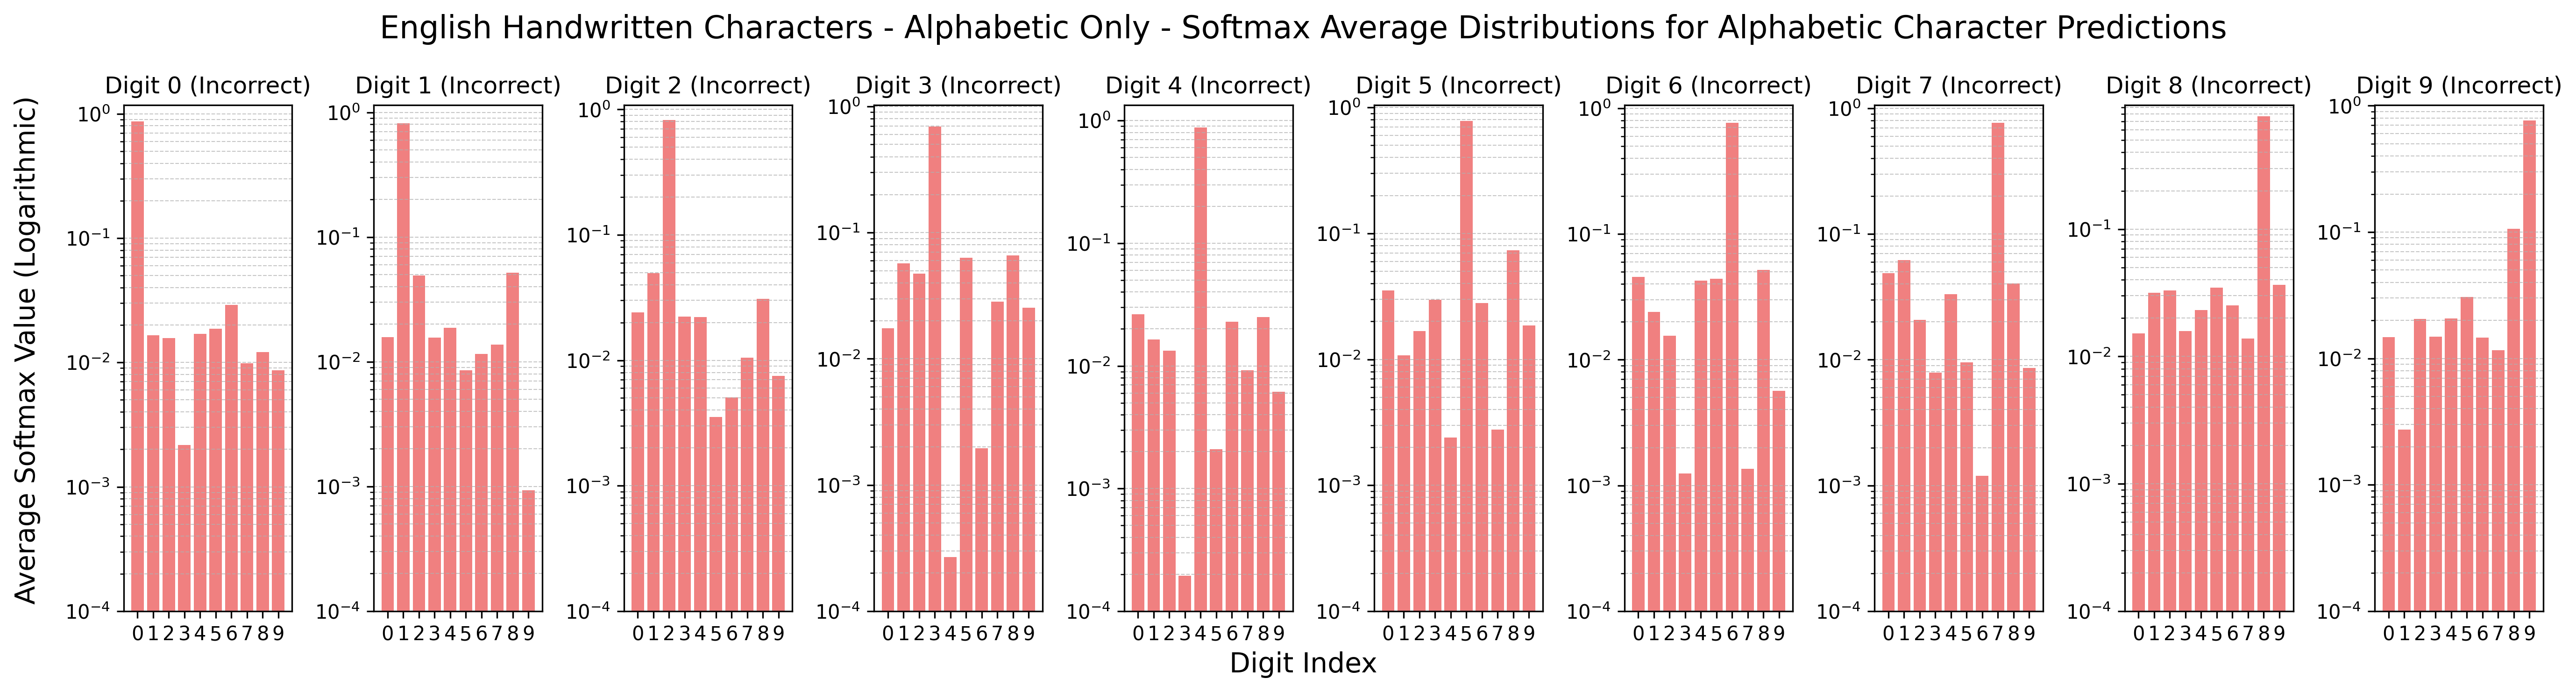
\includegraphics[width=0.99\textwidth]{Figures/Results/HandwrittenCharacters/english_handwritten_characters_alphabetic_softmax_averages.png}
%     \caption{Average Softmax Probabilities for Alphabetic Characters in the English Handwritten Character MNISTified Dataset}
% \label{fig:english_handwritten_characters_alphabetic_softmax_averages}
% \end{figure*}


% \subsection{MNIST, CIFAR-10 Training Dataset Entropy Comparison}

% \begin{figure}[ht]
%     \centering
%     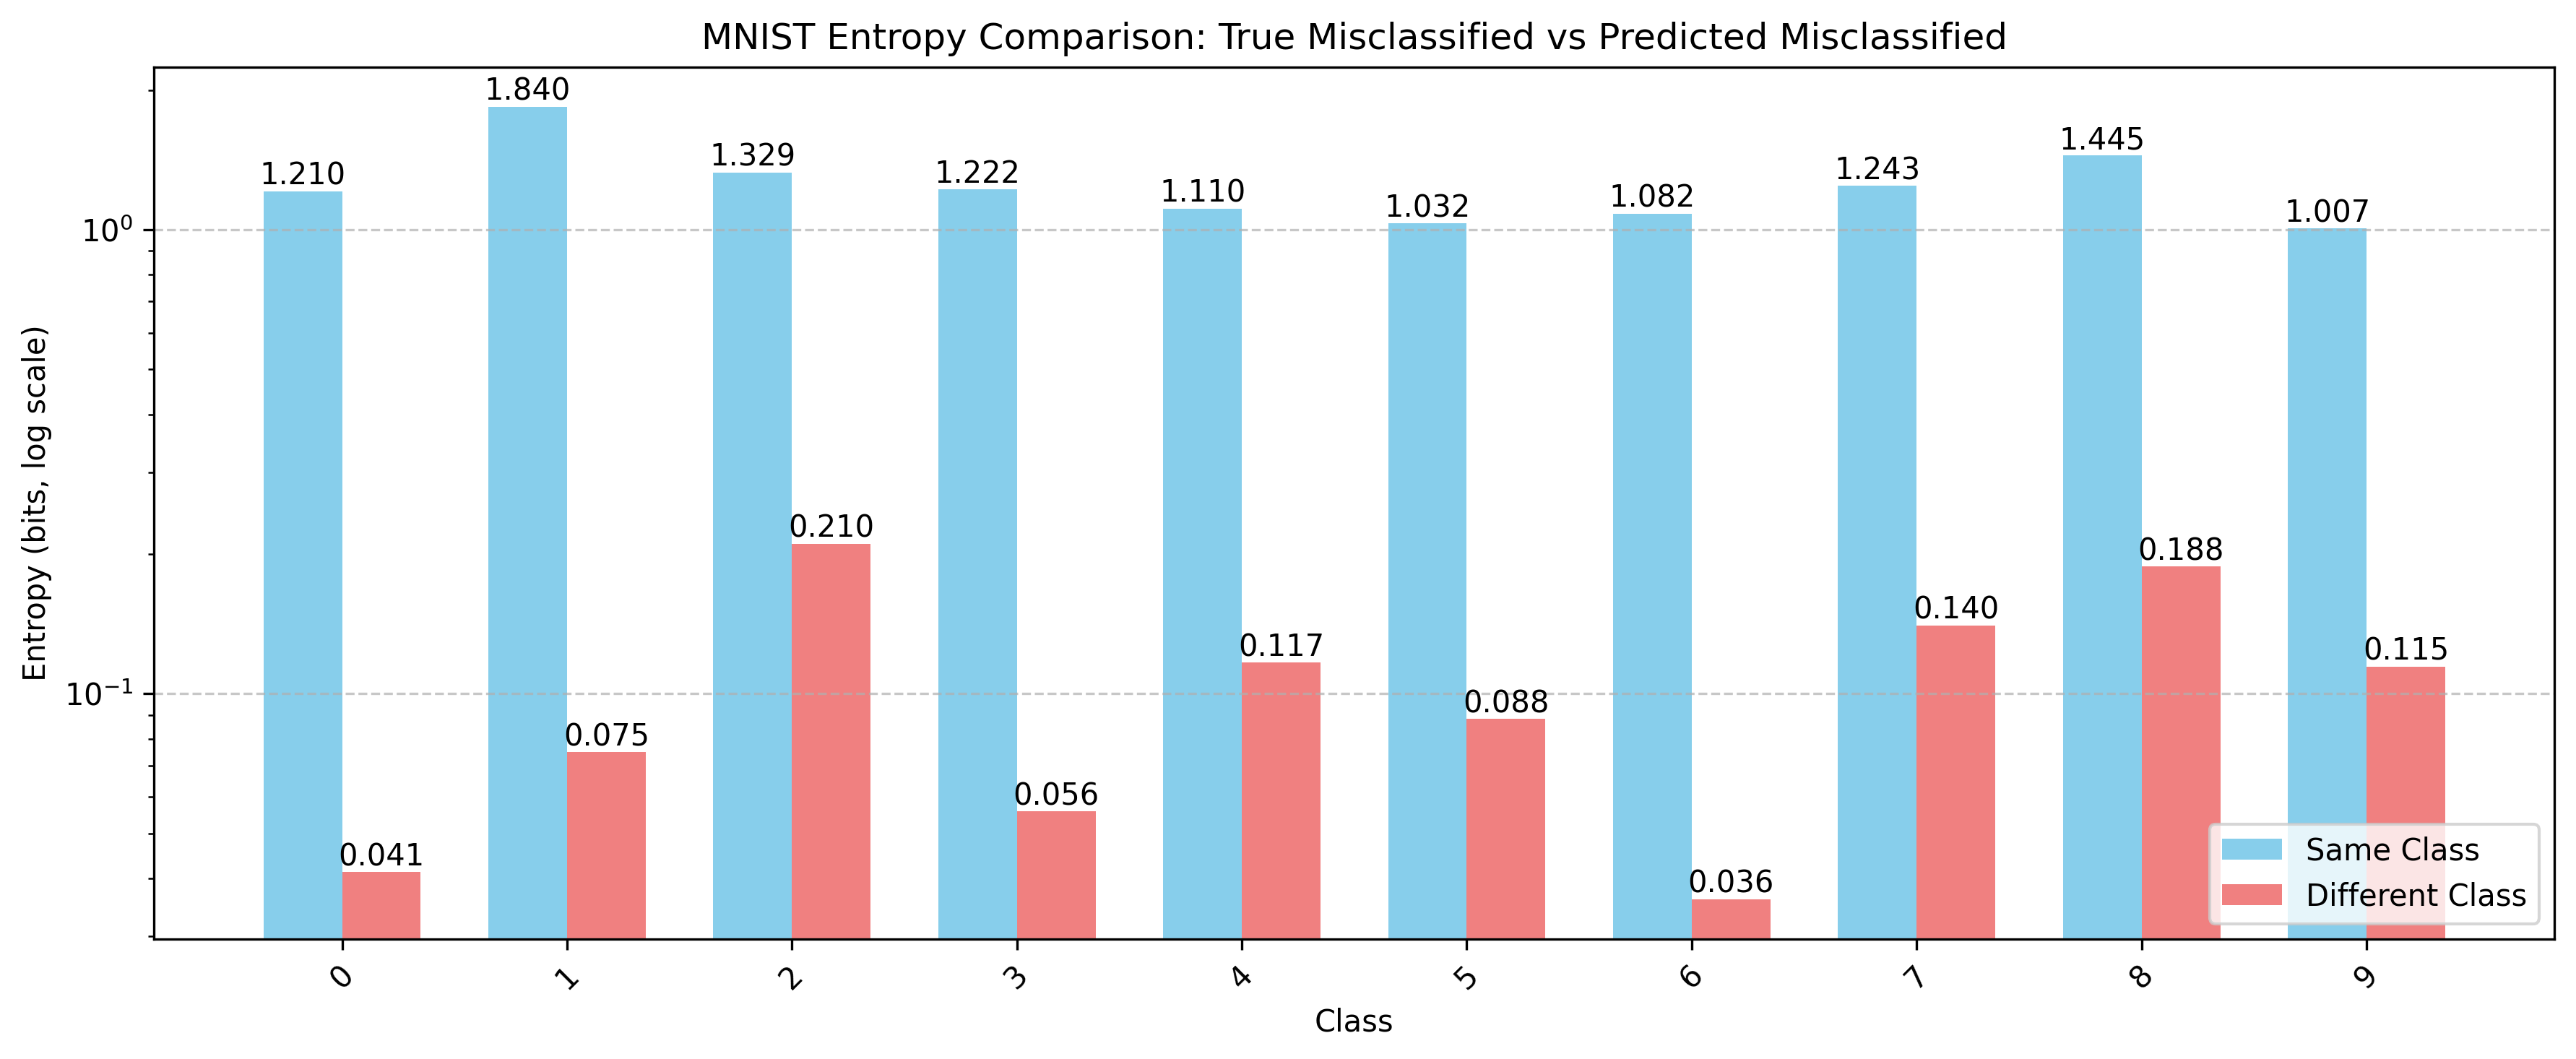
\includegraphics[width=0.99\textwidth]{Figures/Results/HandwrittenCharacters/mnist_entropy_comparison.png}
%     \caption{MNIST entropy values for misclassified example from same class nearest to class centroid (cyan) and nearest misclassified example from different class to class centroid (red).}
% \label{fig:mnist_entropy_comparison}
% \end{figure}

% \begin{figure}[ht]
%     \centering
%     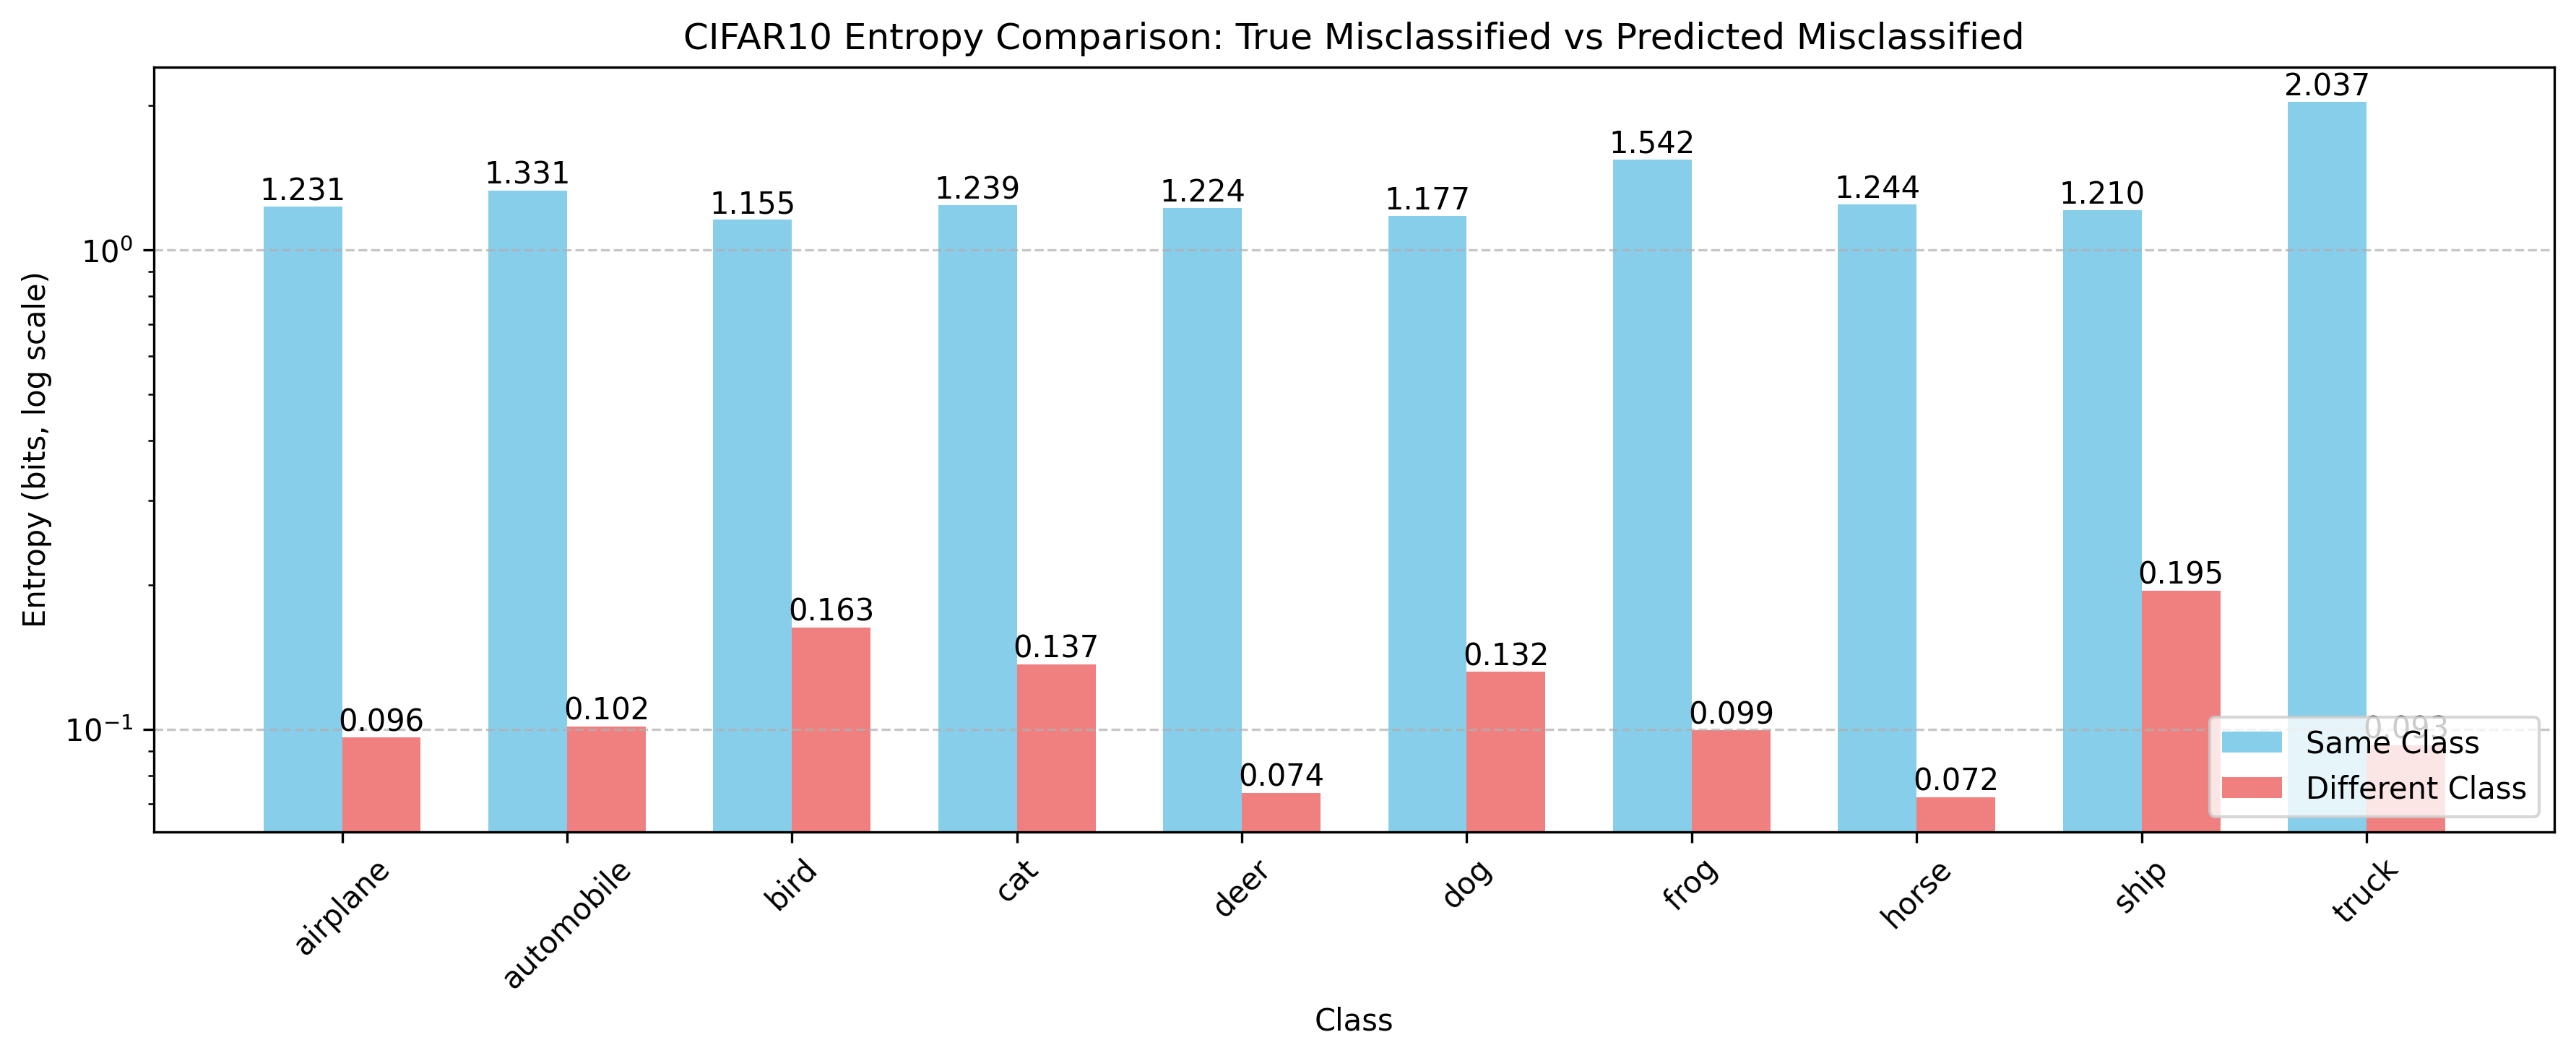
\includegraphics[width=0.99\textwidth]{Figures/Results/HandwrittenCharacters/cifar_vit_entropy_comparison.png}
%     \caption{CIFAR-10 entropy values for misclassified example from same class nearest to class centroid (cyan) and nearest misclassified example from different class to class centroid (red).}
% \label{fig:cifar_vit_entropy_comparison}
% \end{figure}
